\documentclass[oneside,openright,titlepage,numbers=noenddot,headinclude,footinclude=true,cleardoublepage=empty,listof=totoc,paper=a4,fontsize=11pt,english,BCOR=5mm]{scrreprt}

% -----------------------------------------------------------------------------
%   CONFIGURATION
% -----------------------------------------------------------------------------
% Thesis and submission:
\newcommand{\myTitle}{Computer Forensics: Blue Coursework}
\newcommand{\mySubmissionYear}{2021}
\newcommand{\mySubmissionMonth}{December}
\newcommand{\mySubmissionDay}{15}

% My information:
\newcommand{\myFirstName}{Alessandro}
\newcommand{\myLastName}{Buonerba}
\newcommand{\myWebsite}{https://www.linkedin.com/in/buonerba/}

% Module Leader:
\newcommand{\myProfTitle}{Dr}
\newcommand{\myProfFirstName}{David}
\newcommand{\myProfLastName}{Gresty}
\newcommand{\myProfWebsite}{https://www.gre.ac.uk/people/rep/las/david-gresty}

% University related:
\newcommand{\myDepartment}{Department of Computing \& Mathematical Sciences}
\newcommand{\myFaculty}{Liberal Arts \& Sciences}
\newcommand{\myUni}{University of Greenwich}
% -----------------------------------------------------------------------------

% ****************************************************************************************************
% classicthesis-config.tex
% formerly known as loadpackages.sty, classicthesis-ldpkg.sty, and classicthesis-preamble.sty
% Use it at the beginning of your ClassicThesis.tex, or as a LaTeX Preamble
% in your ClassicThesis.{tex,lyx} with % ****************************************************************************************************
% classicthesis-config.tex
% formerly known as loadpackages.sty, classicthesis-ldpkg.sty, and classicthesis-preamble.sty
% Use it at the beginning of your ClassicThesis.tex, or as a LaTeX Preamble
% in your ClassicThesis.{tex,lyx} with % ****************************************************************************************************
% classicthesis-config.tex
% formerly known as loadpackages.sty, classicthesis-ldpkg.sty, and classicthesis-preamble.sty
% Use it at the beginning of your ClassicThesis.tex, or as a LaTeX Preamble
% in your ClassicThesis.{tex,lyx} with \input{classicthesis-config}
% ****************************************************************************************************
% If you like the classicthesis, then I would appreciate a postcard.
% My address can be found in the file ClassicThesis.pdf. A collection
% of the postcards I received so far is available online at
% http://postcards.miede.de

% ****************************************************************************************************
% 0. Set the encoding of your files. UTF-8 is the only sensible encoding nowadays. If you can't read
% äöüßáéçèê∂åëæƒÏ€ then change the encoding setting in your editor, not the line below. If your editor
% does not support utf8 use another editor!
% ****************************************************************************************************
\PassOptionsToPackage{utf8}{inputenc}
  \usepackage{inputenc}


% ****************************************************************************************************
% 1. Configure classicthesis for your needs here, e.g., remove "drafting" below
% in order to deactivate the time-stamp on the pages
% ****************************************************************************************************
\PassOptionsToPackage{eulerchapternumbers,listings,pdfspacing,subfig,beramono,dottedtoc}{classicthesis}
% ********************************************************************
% Available options for classicthesis.sty
% (see ClassicThesis.pdf for more information):
% drafting
% parts nochapters linedheaders
% eulerchapternumbers beramono eulermath pdfspacing minionprospacing
% tocaligned dottedtoc manychapters
% listings floatperchapter subfig
% ********************************************************************


% ****************************************************************************************************
% 2. Personal data and user ad-hoc commands
% ****************************************************************************************************
% moved to thesis.tex


% ********************************************************************
% Setup, finetuning, and useful commands
% ********************************************************************
\newcounter{dummy} % necessary for correct hyperlinks (to index, bib, etc.)
\newlength{\abcd} % for ab..z string length calculation
\providecommand{\mLyX}{L\kern-.1667em\lower.25em\hbox{Y}\kern-.125emX\@}
\newcommand{\ie}{i.\,e.\ }
\newcommand{\Ie}{I.\,e.\ }
\newcommand{\eg}{e.\,g.\ }
\newcommand{\Eg}{E.\,g.\ }
% ****************************************************************************************************


% ****************************************************************************************************
% 3. Loading some handy packages
% ****************************************************************************************************
% ********************************************************************
% Packages with options that might require adjustments
% ********************************************************************
\PassOptionsToPackage{english}{babel}
\usepackage{babel}

\usepackage{csquotes}
\PassOptionsToPackage{%
  backend=bibtex,
  bibencoding=ascii,
  language=auto,
  style=numeric,
  sorting=nyt,
  maxbibnames=10,
  natbib=true
}{biblatex}
\usepackage[style=authoryear]{biblatex}
\usepackage{xurl}
\PassOptionsToPackage{fleqn}{amsmath}       % math environments and more by the AMS
\usepackage{amsmath}

% ********************************************************************
% General useful packages
% ********************************************************************
\usepackage{amssymb}
\usepackage{lipsum}
\PassOptionsToPackage{T1}{fontenc} % T2A for cyrillics
\usepackage{fontenc}
\usepackage{textcomp} % fix warning with missing font shapes
\usepackage{scrhack} % fix warnings when using KOMA with listings package
\usepackage{xspace} % to get the spacing after macros right
\usepackage{mparhack} % get marginpar right
%\usepackage[latest]{latexrelease} % will be used once available in more distributions (ISSUE #107)
\PassOptionsToPackage{printonlyused,smaller}{acronym}
\usepackage{acronym} % nice macros for handling all acronyms in the thesis
%\renewcommand{\bflabel}[1]{{#1}\hfill} % fix the list of acronyms --> no longer working
%\renewcommand*{\acsfont}[1]{\textsc{#1}}
\renewcommand*{\aclabelfont}[1]{\acsfont{#1}}
% ****************************************************************************************************


% ****************************************************************************************************
% 4. Setup floats: tables, (sub)figures, and captions
% ****************************************************************************************************
\usepackage{tabularx} % better tables
\setlength{\extrarowheight}{3pt} % increase table row height
\newcommand{\tableheadline}[1]{\multicolumn{1}{c}{\spacedlowsmallcaps{#1}}}
\newcommand{\myfloatalign}{\centering} % to be used with each float for alignment
\usepackage{makecell}
\usepackage{multirow}
\usepackage{caption}
% Thanks to cgnieder and Claus Lahiri
% http://tex.stackexchange.com/questions/69349/spacedlowsmallcaps-in-caption-label
% [REMOVED DUE TO OTHER PROBLEMS, SEE ISSUE #82]
%\DeclareCaptionLabelFormat{smallcaps}{\bothIfFirst{#1}{~}\MakeTextLowercase{\textsc{#2}}}
%\captionsetup{font=small,labelformat=smallcaps} % format=hang,
\captionsetup{font=small} % format=hang,
\usepackage{subfig}
% ****************************************************************************************************


% ****************************************************************************************************
% 5. Setup code listings
% ****************************************************************************************************
\usepackage{listings}
%\lstset{emph={trueIndex,root},emphstyle=\color{BlueViolet}}%\underbar} % For special keywords
\lstset{language=[LaTeX]Tex,%C++,
  morekeywords={PassOptionsToPackage,selectlanguage},
  keywordstyle=\color{RoyalBlue},%\bfseries,
  basicstyle=\small\ttfamily,
  %identifierstyle=\color{NavyBlue},
  commentstyle=\color{Green}\ttfamily,
  stringstyle=\rmfamily,
  numbers=left,
  numberstyle=\scriptsize,%\tiny
  stepnumber=5,
  numbersep=8pt,
  showstringspaces=false,
  breaklines=true,
  %frameround=ftff,
  %frame=single,
  belowcaptionskip=.75\baselineskip{}
  %frame=L
}
% ****************************************************************************************************


% ****************************************************************************************************
% 6. PDFLaTeX, hyperreferences and citation backreferences
% ****************************************************************************************************
% ********************************************************************
% Using PDFLaTeX
% ********************************************************************
\PassOptionsToPackage{pdftex,hyperfootnotes=false,pdfpagelabels}{hyperref}
\usepackage{hyperref}  % backref linktocpage pagebackref
\pdfcompresslevel=9
\pdfadjustspacing=1
\PassOptionsToPackage{pdftex}{graphicx}
    \usepackage{graphicx}


% ********************************************************************
% Hyperreferences
% ********************************************************************
\hypersetup{breaklinks=true}
\hypersetup{linktocpage=true}
\hypersetup{colorlinks=true}
\hypersetup{urlcolor=RoyalBlue}
\hypersetup{linkcolor=RoyalBlue}
\hypersetup{citecolor=webgreen}
\hypersetup{pageanchor=true}
\hypersetup{plainpages=false}
%\hypersetup{bookmarksnumbered=true}
%\hypersetup{bookmarksopen=true}
%\hypersetup{bookmarksopenlevel=true}
%hypertexnames=true, nesting=true, frenchlinks
\hypersetup{pdfstartpage=3}
\hypersetup{pdfstartview=FitV}
\hypersetup{pdfpagemode=UseNone}
\hypersetup{pageanchor=true}
\hypersetup{pdfpagemode=UseOutlines}
\hypersetup{pdftitle={\myTitle}}
\hypersetup{pdfauthor={\textcopyright\ \myFirstName\ \myLastName, \myUni, \myFaculty}}
\hypersetup{pdfsubject={}}
\hypersetup{pdfkeywords={}}
\hypersetup{pdfhighlight=/O}


% ********************************************************************
% Setup autoreferences
% ********************************************************************
% There are some issues regarding autorefnames
% http://www.ureader.de/msg/136221647.aspx
% http://www.tex.ac.uk/cgi-bin/texfaq2html?label=latexwords
% you have to redefine the makros for the
% language you use, e.g., american, ngerman
% (as chosen when loading babel/AtBeginDocument)
% ********************************************************************
\makeatletter
\@ifpackageloaded{babel}%
{%
  \addto\extrasenglish{%
    \renewcommand*{\figureautorefname}{Figure}%
    \renewcommand*{\tableautorefname}{Table}%
    \renewcommand*{\partautorefname}{Part}%
    \renewcommand*{\chapterautorefname}{Chapter}%
    \renewcommand*{\sectionautorefname}{Section}%
    \renewcommand*{\subsectionautorefname}{Section}%
    \renewcommand*{\subsubsectionautorefname}{Section}%
  }%
  \addto\extrasngerman{%
    \renewcommand*{\paragraphautorefname}{Absatz}%
    \renewcommand*{\subparagraphautorefname}{Unterabsatz}%
    \renewcommand*{\footnoteautorefname}{Fu\"snote}%
    \renewcommand*{\FancyVerbLineautorefname}{Zeile}%
    \renewcommand*{\theoremautorefname}{Theorem}%
    \renewcommand*{\appendixautorefname}{Anhang}%
    \renewcommand*{\equationautorefname}{Gleichung}%
    \renewcommand*{\itemautorefname}{Punkt}%
  }%
  % Fix to getting autorefs for subfigures right (thanks to Belinda Vogt for changing the definition)
  \providecommand{\subfigureautorefname}{\figureautorefname}%
}{\relax}
\makeatother


% ****************************************************************************************************
% 7. Last calls before the bar closes
% ****************************************************************************************************
% ********************************************************************
% Development Stuff
% ********************************************************************
%\listfiles
%\PassOptionsToPackage{l2tabu,orthodox,abort}{nag}
%   \usepackage{nag}
%\PassOptionsToPackage{warning, all}{onlyamsmath}
%   \usepackage{onlyamsmath}

% ********************************************************************
% Last, but not least...
% ********************************************************************
\usepackage{classicthesis}
% ****************************************************************************************************


% ****************************************************************************************************
% 8. Further adjustments (experimental)
% ****************************************************************************************************
% ********************************************************************
% Changing the text area
% ********************************************************************
%\linespread{1.05} % a bit more for Palatino
%\areaset[current]{312pt}{761pt} % 686 (factor 2.2) + 33 head + 42 head \the\footskip
%\setlength{\marginparwidth}{7em}%
%\setlength{\marginparsep}{2em}%

% ********************************************************************
% Using different fonts
% ********************************************************************
%\usepackage[oldstylenums]{kpfonts} % oldstyle notextcomp
%\usepackage[osf]{libertine}
%\usepackage[light,condensed,math]{iwona}
%\renewcommand{\sfdefault}{iwona}
%\usepackage{lmodern} % <-- no osf support :-(
%\usepackage{cfr-lm} %
%\usepackage[urw-garamond]{mathdesign} <-- no osf support :-(
%\usepackage[default,osfigures]{opensans} % scale=0.95
%\usepackage[sfdefault]{FiraSans}
% ****************************************************************************************************


% ****************************************************************************************************
% 9. LTU Extensions
% ****************************************************************************************************
\usepackage{colortbl}
\usepackage{setspace}
\usepackage{fp}
\usepackage{soul}

\usepackage{textcomp}

\usepackage{pgfplots}
\usepackage{pgfplotstable}
\pgfplotsset{compat=newest}

\usepackage[shortcuts]{extdash}
%\usepackage{epigraph}

\usepackage{tikz-timing}[2011/01/09]
\usetikzlibrary{arrows, backgrounds, patterns, shapes}
\usepackage{arydshln}

\usepackage{algorithm}
\usepackage{algorithmic}
\newcommand{\algorithmautorefname}{Algorithm}

\renewcommand{\lstlistlistingname}{List of Listings}

\DeclareMathOperator*{\argmin}{argmin}
\DeclareMathOperator*{\argmax}{argmax}

\renewcommand{\rmdefault}{pnc}
\renewcommand{\rmdefault}{pplx}

\newcolumntype{L}[1]{>{\raggedright\arraybackslash}m{#1}}
\newcolumntype{C}[1]{>{\centering\arraybackslash}m{#1}}
\newcolumntype{R}[1]{>{\raggedleft\arraybackslash}m{#1}}

\numberwithin{equation}{chapter}
\numberwithin{figure}{chapter}
\numberwithin{table}{chapter}
\numberwithin{algorithm}{chapter}
\sloppy

\renewcommand{\bibfont}{\footnotesize}

\newcommand{\hinttext}[1]{\textcolor{Gray!70!Red}{#1}}

% ****************************************************************************************************

% ****************************************************************************************************
% If you like the classicthesis, then I would appreciate a postcard.
% My address can be found in the file ClassicThesis.pdf. A collection
% of the postcards I received so far is available online at
% http://postcards.miede.de

% ****************************************************************************************************
% 0. Set the encoding of your files. UTF-8 is the only sensible encoding nowadays. If you can't read
% äöüßáéçèê∂åëæƒÏ€ then change the encoding setting in your editor, not the line below. If your editor
% does not support utf8 use another editor!
% ****************************************************************************************************
\PassOptionsToPackage{utf8}{inputenc}
  \usepackage{inputenc}


% ****************************************************************************************************
% 1. Configure classicthesis for your needs here, e.g., remove "drafting" below
% in order to deactivate the time-stamp on the pages
% ****************************************************************************************************
\PassOptionsToPackage{eulerchapternumbers,listings,pdfspacing,subfig,beramono,dottedtoc}{classicthesis}
% ********************************************************************
% Available options for classicthesis.sty
% (see ClassicThesis.pdf for more information):
% drafting
% parts nochapters linedheaders
% eulerchapternumbers beramono eulermath pdfspacing minionprospacing
% tocaligned dottedtoc manychapters
% listings floatperchapter subfig
% ********************************************************************


% ****************************************************************************************************
% 2. Personal data and user ad-hoc commands
% ****************************************************************************************************
% moved to thesis.tex


% ********************************************************************
% Setup, finetuning, and useful commands
% ********************************************************************
\newcounter{dummy} % necessary for correct hyperlinks (to index, bib, etc.)
\newlength{\abcd} % for ab..z string length calculation
\providecommand{\mLyX}{L\kern-.1667em\lower.25em\hbox{Y}\kern-.125emX\@}
\newcommand{\ie}{i.\,e.\ }
\newcommand{\Ie}{I.\,e.\ }
\newcommand{\eg}{e.\,g.\ }
\newcommand{\Eg}{E.\,g.\ }
% ****************************************************************************************************


% ****************************************************************************************************
% 3. Loading some handy packages
% ****************************************************************************************************
% ********************************************************************
% Packages with options that might require adjustments
% ********************************************************************
\PassOptionsToPackage{english}{babel}
\usepackage{babel}

\usepackage{csquotes}
\PassOptionsToPackage{%
  backend=bibtex,
  bibencoding=ascii,
  language=auto,
  style=numeric,
  sorting=nyt,
  maxbibnames=10,
  natbib=true
}{biblatex}
\usepackage[style=authoryear]{biblatex}
\usepackage{xurl}
\PassOptionsToPackage{fleqn}{amsmath}       % math environments and more by the AMS
\usepackage{amsmath}

% ********************************************************************
% General useful packages
% ********************************************************************
\usepackage{amssymb}
\usepackage{lipsum}
\PassOptionsToPackage{T1}{fontenc} % T2A for cyrillics
\usepackage{fontenc}
\usepackage{textcomp} % fix warning with missing font shapes
\usepackage{scrhack} % fix warnings when using KOMA with listings package
\usepackage{xspace} % to get the spacing after macros right
\usepackage{mparhack} % get marginpar right
%\usepackage[latest]{latexrelease} % will be used once available in more distributions (ISSUE #107)
\PassOptionsToPackage{printonlyused,smaller}{acronym}
\usepackage{acronym} % nice macros for handling all acronyms in the thesis
%\renewcommand{\bflabel}[1]{{#1}\hfill} % fix the list of acronyms --> no longer working
%\renewcommand*{\acsfont}[1]{\textsc{#1}}
\renewcommand*{\aclabelfont}[1]{\acsfont{#1}}
% ****************************************************************************************************


% ****************************************************************************************************
% 4. Setup floats: tables, (sub)figures, and captions
% ****************************************************************************************************
\usepackage{tabularx} % better tables
\setlength{\extrarowheight}{3pt} % increase table row height
\newcommand{\tableheadline}[1]{\multicolumn{1}{c}{\spacedlowsmallcaps{#1}}}
\newcommand{\myfloatalign}{\centering} % to be used with each float for alignment
\usepackage{makecell}
\usepackage{multirow}
\usepackage{caption}
% Thanks to cgnieder and Claus Lahiri
% http://tex.stackexchange.com/questions/69349/spacedlowsmallcaps-in-caption-label
% [REMOVED DUE TO OTHER PROBLEMS, SEE ISSUE #82]
%\DeclareCaptionLabelFormat{smallcaps}{\bothIfFirst{#1}{~}\MakeTextLowercase{\textsc{#2}}}
%\captionsetup{font=small,labelformat=smallcaps} % format=hang,
\captionsetup{font=small} % format=hang,
\usepackage{subfig}
% ****************************************************************************************************


% ****************************************************************************************************
% 5. Setup code listings
% ****************************************************************************************************
\usepackage{listings}
%\lstset{emph={trueIndex,root},emphstyle=\color{BlueViolet}}%\underbar} % For special keywords
\lstset{language=[LaTeX]Tex,%C++,
  morekeywords={PassOptionsToPackage,selectlanguage},
  keywordstyle=\color{RoyalBlue},%\bfseries,
  basicstyle=\small\ttfamily,
  %identifierstyle=\color{NavyBlue},
  commentstyle=\color{Green}\ttfamily,
  stringstyle=\rmfamily,
  numbers=left,
  numberstyle=\scriptsize,%\tiny
  stepnumber=5,
  numbersep=8pt,
  showstringspaces=false,
  breaklines=true,
  %frameround=ftff,
  %frame=single,
  belowcaptionskip=.75\baselineskip{}
  %frame=L
}
% ****************************************************************************************************


% ****************************************************************************************************
% 6. PDFLaTeX, hyperreferences and citation backreferences
% ****************************************************************************************************
% ********************************************************************
% Using PDFLaTeX
% ********************************************************************
\PassOptionsToPackage{pdftex,hyperfootnotes=false,pdfpagelabels}{hyperref}
\usepackage{hyperref}  % backref linktocpage pagebackref
\pdfcompresslevel=9
\pdfadjustspacing=1
\PassOptionsToPackage{pdftex}{graphicx}
    \usepackage{graphicx}


% ********************************************************************
% Hyperreferences
% ********************************************************************
\hypersetup{breaklinks=true}
\hypersetup{linktocpage=true}
\hypersetup{colorlinks=true}
\hypersetup{urlcolor=RoyalBlue}
\hypersetup{linkcolor=RoyalBlue}
\hypersetup{citecolor=webgreen}
\hypersetup{pageanchor=true}
\hypersetup{plainpages=false}
%\hypersetup{bookmarksnumbered=true}
%\hypersetup{bookmarksopen=true}
%\hypersetup{bookmarksopenlevel=true}
%hypertexnames=true, nesting=true, frenchlinks
\hypersetup{pdfstartpage=3}
\hypersetup{pdfstartview=FitV}
\hypersetup{pdfpagemode=UseNone}
\hypersetup{pageanchor=true}
\hypersetup{pdfpagemode=UseOutlines}
\hypersetup{pdftitle={\myTitle}}
\hypersetup{pdfauthor={\textcopyright\ \myFirstName\ \myLastName, \myUni, \myFaculty}}
\hypersetup{pdfsubject={}}
\hypersetup{pdfkeywords={}}
\hypersetup{pdfhighlight=/O}


% ********************************************************************
% Setup autoreferences
% ********************************************************************
% There are some issues regarding autorefnames
% http://www.ureader.de/msg/136221647.aspx
% http://www.tex.ac.uk/cgi-bin/texfaq2html?label=latexwords
% you have to redefine the makros for the
% language you use, e.g., american, ngerman
% (as chosen when loading babel/AtBeginDocument)
% ********************************************************************
\makeatletter
\@ifpackageloaded{babel}%
{%
  \addto\extrasenglish{%
    \renewcommand*{\figureautorefname}{Figure}%
    \renewcommand*{\tableautorefname}{Table}%
    \renewcommand*{\partautorefname}{Part}%
    \renewcommand*{\chapterautorefname}{Chapter}%
    \renewcommand*{\sectionautorefname}{Section}%
    \renewcommand*{\subsectionautorefname}{Section}%
    \renewcommand*{\subsubsectionautorefname}{Section}%
  }%
  \addto\extrasngerman{%
    \renewcommand*{\paragraphautorefname}{Absatz}%
    \renewcommand*{\subparagraphautorefname}{Unterabsatz}%
    \renewcommand*{\footnoteautorefname}{Fu\"snote}%
    \renewcommand*{\FancyVerbLineautorefname}{Zeile}%
    \renewcommand*{\theoremautorefname}{Theorem}%
    \renewcommand*{\appendixautorefname}{Anhang}%
    \renewcommand*{\equationautorefname}{Gleichung}%
    \renewcommand*{\itemautorefname}{Punkt}%
  }%
  % Fix to getting autorefs for subfigures right (thanks to Belinda Vogt for changing the definition)
  \providecommand{\subfigureautorefname}{\figureautorefname}%
}{\relax}
\makeatother


% ****************************************************************************************************
% 7. Last calls before the bar closes
% ****************************************************************************************************
% ********************************************************************
% Development Stuff
% ********************************************************************
%\listfiles
%\PassOptionsToPackage{l2tabu,orthodox,abort}{nag}
%   \usepackage{nag}
%\PassOptionsToPackage{warning, all}{onlyamsmath}
%   \usepackage{onlyamsmath}

% ********************************************************************
% Last, but not least...
% ********************************************************************
\usepackage{classicthesis}
% ****************************************************************************************************


% ****************************************************************************************************
% 8. Further adjustments (experimental)
% ****************************************************************************************************
% ********************************************************************
% Changing the text area
% ********************************************************************
%\linespread{1.05} % a bit more for Palatino
%\areaset[current]{312pt}{761pt} % 686 (factor 2.2) + 33 head + 42 head \the\footskip
%\setlength{\marginparwidth}{7em}%
%\setlength{\marginparsep}{2em}%

% ********************************************************************
% Using different fonts
% ********************************************************************
%\usepackage[oldstylenums]{kpfonts} % oldstyle notextcomp
%\usepackage[osf]{libertine}
%\usepackage[light,condensed,math]{iwona}
%\renewcommand{\sfdefault}{iwona}
%\usepackage{lmodern} % <-- no osf support :-(
%\usepackage{cfr-lm} %
%\usepackage[urw-garamond]{mathdesign} <-- no osf support :-(
%\usepackage[default,osfigures]{opensans} % scale=0.95
%\usepackage[sfdefault]{FiraSans}
% ****************************************************************************************************


% ****************************************************************************************************
% 9. LTU Extensions
% ****************************************************************************************************
\usepackage{colortbl}
\usepackage{setspace}
\usepackage{fp}
\usepackage{soul}

\usepackage{textcomp}

\usepackage{pgfplots}
\usepackage{pgfplotstable}
\pgfplotsset{compat=newest}

\usepackage[shortcuts]{extdash}
%\usepackage{epigraph}

\usepackage{tikz-timing}[2011/01/09]
\usetikzlibrary{arrows, backgrounds, patterns, shapes}
\usepackage{arydshln}

\usepackage{algorithm}
\usepackage{algorithmic}
\newcommand{\algorithmautorefname}{Algorithm}

\renewcommand{\lstlistlistingname}{List of Listings}

\DeclareMathOperator*{\argmin}{argmin}
\DeclareMathOperator*{\argmax}{argmax}

\renewcommand{\rmdefault}{pnc}
\renewcommand{\rmdefault}{pplx}

\newcolumntype{L}[1]{>{\raggedright\arraybackslash}m{#1}}
\newcolumntype{C}[1]{>{\centering\arraybackslash}m{#1}}
\newcolumntype{R}[1]{>{\raggedleft\arraybackslash}m{#1}}

\numberwithin{equation}{chapter}
\numberwithin{figure}{chapter}
\numberwithin{table}{chapter}
\numberwithin{algorithm}{chapter}
\sloppy

\renewcommand{\bibfont}{\footnotesize}

\newcommand{\hinttext}[1]{\textcolor{Gray!70!Red}{#1}}

% ****************************************************************************************************

% ****************************************************************************************************
% If you like the classicthesis, then I would appreciate a postcard.
% My address can be found in the file ClassicThesis.pdf. A collection
% of the postcards I received so far is available online at
% http://postcards.miede.de

% ****************************************************************************************************
% 0. Set the encoding of your files. UTF-8 is the only sensible encoding nowadays. If you can't read
% äöüßáéçèê∂åëæƒÏ€ then change the encoding setting in your editor, not the line below. If your editor
% does not support utf8 use another editor!
% ****************************************************************************************************
\PassOptionsToPackage{utf8}{inputenc}
  \usepackage{inputenc}


% ****************************************************************************************************
% 1. Configure classicthesis for your needs here, e.g., remove "drafting" below
% in order to deactivate the time-stamp on the pages
% ****************************************************************************************************
\PassOptionsToPackage{eulerchapternumbers,listings,pdfspacing,subfig,beramono,dottedtoc}{classicthesis}
% ********************************************************************
% Available options for classicthesis.sty
% (see ClassicThesis.pdf for more information):
% drafting
% parts nochapters linedheaders
% eulerchapternumbers beramono eulermath pdfspacing minionprospacing
% tocaligned dottedtoc manychapters
% listings floatperchapter subfig
% ********************************************************************


% ****************************************************************************************************
% 2. Personal data and user ad-hoc commands
% ****************************************************************************************************
% moved to thesis.tex


% ********************************************************************
% Setup, finetuning, and useful commands
% ********************************************************************
\newcounter{dummy} % necessary for correct hyperlinks (to index, bib, etc.)
\newlength{\abcd} % for ab..z string length calculation
\providecommand{\mLyX}{L\kern-.1667em\lower.25em\hbox{Y}\kern-.125emX\@}
\newcommand{\ie}{i.\,e.\ }
\newcommand{\Ie}{I.\,e.\ }
\newcommand{\eg}{e.\,g.\ }
\newcommand{\Eg}{E.\,g.\ }
% ****************************************************************************************************


% ****************************************************************************************************
% 3. Loading some handy packages
% ****************************************************************************************************
% ********************************************************************
% Packages with options that might require adjustments
% ********************************************************************
\PassOptionsToPackage{english}{babel}
\usepackage{babel}

\usepackage{csquotes}
\PassOptionsToPackage{%
  backend=bibtex,
  bibencoding=ascii,
  language=auto,
  style=numeric,
  sorting=nyt,
  maxbibnames=10,
  natbib=true
}{biblatex}
\usepackage[style=authoryear]{biblatex}
\usepackage{xurl}
\PassOptionsToPackage{fleqn}{amsmath}       % math environments and more by the AMS
\usepackage{amsmath}

% ********************************************************************
% General useful packages
% ********************************************************************
\usepackage{amssymb}
\usepackage{lipsum}
\PassOptionsToPackage{T1}{fontenc} % T2A for cyrillics
\usepackage{fontenc}
\usepackage{textcomp} % fix warning with missing font shapes
\usepackage{scrhack} % fix warnings when using KOMA with listings package
\usepackage{xspace} % to get the spacing after macros right
\usepackage{mparhack} % get marginpar right
%\usepackage[latest]{latexrelease} % will be used once available in more distributions (ISSUE #107)
\PassOptionsToPackage{printonlyused,smaller}{acronym}
\usepackage{acronym} % nice macros for handling all acronyms in the thesis
%\renewcommand{\bflabel}[1]{{#1}\hfill} % fix the list of acronyms --> no longer working
%\renewcommand*{\acsfont}[1]{\textsc{#1}}
\renewcommand*{\aclabelfont}[1]{\acsfont{#1}}
% ****************************************************************************************************


% ****************************************************************************************************
% 4. Setup floats: tables, (sub)figures, and captions
% ****************************************************************************************************
\usepackage{tabularx} % better tables
\setlength{\extrarowheight}{3pt} % increase table row height
\newcommand{\tableheadline}[1]{\multicolumn{1}{c}{\spacedlowsmallcaps{#1}}}
\newcommand{\myfloatalign}{\centering} % to be used with each float for alignment
\usepackage{makecell}
\usepackage{multirow}
\usepackage{caption}
% Thanks to cgnieder and Claus Lahiri
% http://tex.stackexchange.com/questions/69349/spacedlowsmallcaps-in-caption-label
% [REMOVED DUE TO OTHER PROBLEMS, SEE ISSUE #82]
%\DeclareCaptionLabelFormat{smallcaps}{\bothIfFirst{#1}{~}\MakeTextLowercase{\textsc{#2}}}
%\captionsetup{font=small,labelformat=smallcaps} % format=hang,
\captionsetup{font=small} % format=hang,
\usepackage{subfig}
% ****************************************************************************************************


% ****************************************************************************************************
% 5. Setup code listings
% ****************************************************************************************************
\usepackage{listings}
%\lstset{emph={trueIndex,root},emphstyle=\color{BlueViolet}}%\underbar} % For special keywords
\lstset{language=[LaTeX]Tex,%C++,
  morekeywords={PassOptionsToPackage,selectlanguage},
  keywordstyle=\color{RoyalBlue},%\bfseries,
  basicstyle=\small\ttfamily,
  %identifierstyle=\color{NavyBlue},
  commentstyle=\color{Green}\ttfamily,
  stringstyle=\rmfamily,
  numbers=left,
  numberstyle=\scriptsize,%\tiny
  stepnumber=5,
  numbersep=8pt,
  showstringspaces=false,
  breaklines=true,
  %frameround=ftff,
  %frame=single,
  belowcaptionskip=.75\baselineskip{}
  %frame=L
}
% ****************************************************************************************************


% ****************************************************************************************************
% 6. PDFLaTeX, hyperreferences and citation backreferences
% ****************************************************************************************************
% ********************************************************************
% Using PDFLaTeX
% ********************************************************************
\PassOptionsToPackage{pdftex,hyperfootnotes=false,pdfpagelabels}{hyperref}
\usepackage{hyperref}  % backref linktocpage pagebackref
\pdfcompresslevel=9
\pdfadjustspacing=1
\PassOptionsToPackage{pdftex}{graphicx}
    \usepackage{graphicx}


% ********************************************************************
% Hyperreferences
% ********************************************************************
\hypersetup{breaklinks=true}
\hypersetup{linktocpage=true}
\hypersetup{colorlinks=true}
\hypersetup{urlcolor=RoyalBlue}
\hypersetup{linkcolor=RoyalBlue}
\hypersetup{citecolor=webgreen}
\hypersetup{pageanchor=true}
\hypersetup{plainpages=false}
%\hypersetup{bookmarksnumbered=true}
%\hypersetup{bookmarksopen=true}
%\hypersetup{bookmarksopenlevel=true}
%hypertexnames=true, nesting=true, frenchlinks
\hypersetup{pdfstartpage=3}
\hypersetup{pdfstartview=FitV}
\hypersetup{pdfpagemode=UseNone}
\hypersetup{pageanchor=true}
\hypersetup{pdfpagemode=UseOutlines}
\hypersetup{pdftitle={\myTitle}}
\hypersetup{pdfauthor={\textcopyright\ \myFirstName\ \myLastName, \myUni, \myFaculty}}
\hypersetup{pdfsubject={}}
\hypersetup{pdfkeywords={}}
\hypersetup{pdfhighlight=/O}


% ********************************************************************
% Setup autoreferences
% ********************************************************************
% There are some issues regarding autorefnames
% http://www.ureader.de/msg/136221647.aspx
% http://www.tex.ac.uk/cgi-bin/texfaq2html?label=latexwords
% you have to redefine the makros for the
% language you use, e.g., american, ngerman
% (as chosen when loading babel/AtBeginDocument)
% ********************************************************************
\makeatletter
\@ifpackageloaded{babel}%
{%
  \addto\extrasenglish{%
    \renewcommand*{\figureautorefname}{Figure}%
    \renewcommand*{\tableautorefname}{Table}%
    \renewcommand*{\partautorefname}{Part}%
    \renewcommand*{\chapterautorefname}{Chapter}%
    \renewcommand*{\sectionautorefname}{Section}%
    \renewcommand*{\subsectionautorefname}{Section}%
    \renewcommand*{\subsubsectionautorefname}{Section}%
  }%
  \addto\extrasngerman{%
    \renewcommand*{\paragraphautorefname}{Absatz}%
    \renewcommand*{\subparagraphautorefname}{Unterabsatz}%
    \renewcommand*{\footnoteautorefname}{Fu\"snote}%
    \renewcommand*{\FancyVerbLineautorefname}{Zeile}%
    \renewcommand*{\theoremautorefname}{Theorem}%
    \renewcommand*{\appendixautorefname}{Anhang}%
    \renewcommand*{\equationautorefname}{Gleichung}%
    \renewcommand*{\itemautorefname}{Punkt}%
  }%
  % Fix to getting autorefs for subfigures right (thanks to Belinda Vogt for changing the definition)
  \providecommand{\subfigureautorefname}{\figureautorefname}%
}{\relax}
\makeatother


% ****************************************************************************************************
% 7. Last calls before the bar closes
% ****************************************************************************************************
% ********************************************************************
% Development Stuff
% ********************************************************************
%\listfiles
%\PassOptionsToPackage{l2tabu,orthodox,abort}{nag}
%   \usepackage{nag}
%\PassOptionsToPackage{warning, all}{onlyamsmath}
%   \usepackage{onlyamsmath}

% ********************************************************************
% Last, but not least...
% ********************************************************************
\usepackage{classicthesis}
% ****************************************************************************************************


% ****************************************************************************************************
% 8. Further adjustments (experimental)
% ****************************************************************************************************
% ********************************************************************
% Changing the text area
% ********************************************************************
%\linespread{1.05} % a bit more for Palatino
%\areaset[current]{312pt}{761pt} % 686 (factor 2.2) + 33 head + 42 head \the\footskip
%\setlength{\marginparwidth}{7em}%
%\setlength{\marginparsep}{2em}%

% ********************************************************************
% Using different fonts
% ********************************************************************
%\usepackage[oldstylenums]{kpfonts} % oldstyle notextcomp
%\usepackage[osf]{libertine}
%\usepackage[light,condensed,math]{iwona}
%\renewcommand{\sfdefault}{iwona}
%\usepackage{lmodern} % <-- no osf support :-(
%\usepackage{cfr-lm} %
%\usepackage[urw-garamond]{mathdesign} <-- no osf support :-(
%\usepackage[default,osfigures]{opensans} % scale=0.95
%\usepackage[sfdefault]{FiraSans}
% ****************************************************************************************************


% ****************************************************************************************************
% 9. LTU Extensions
% ****************************************************************************************************
\usepackage{colortbl}
\usepackage{setspace}
\usepackage{fp}
\usepackage{soul}

\usepackage{textcomp}

\usepackage{pgfplots}
\usepackage{pgfplotstable}
\pgfplotsset{compat=newest}

\usepackage[shortcuts]{extdash}
%\usepackage{epigraph}

\usepackage{tikz-timing}[2011/01/09]
\usetikzlibrary{arrows, backgrounds, patterns, shapes}
\usepackage{arydshln}

\usepackage{algorithm}
\usepackage{algorithmic}
\newcommand{\algorithmautorefname}{Algorithm}

\renewcommand{\lstlistlistingname}{List of Listings}

\DeclareMathOperator*{\argmin}{argmin}
\DeclareMathOperator*{\argmax}{argmax}

\renewcommand{\rmdefault}{pnc}
\renewcommand{\rmdefault}{pplx}

\newcolumntype{L}[1]{>{\raggedright\arraybackslash}m{#1}}
\newcolumntype{C}[1]{>{\centering\arraybackslash}m{#1}}
\newcolumntype{R}[1]{>{\raggedleft\arraybackslash}m{#1}}

\numberwithin{equation}{chapter}
\numberwithin{figure}{chapter}
\numberwithin{table}{chapter}
\numberwithin{algorithm}{chapter}
\sloppy

\renewcommand{\bibfont}{\footnotesize}

\newcommand{\hinttext}[1]{\textcolor{Gray!70!Red}{#1}}

% ****************************************************************************************************

\addbibresource{library.bib}

\begin{document}
  \frenchspacing
  \raggedbottom{}
  \selectlanguage{english}

  \pagestyle{plain}
  \pagenumbering{roman}

  \singlespacing{}
  \begin{titlepage}
  \doublespacing
  \large
  \hfill
  \vfill
  \vspace*{0.5cm}
  \begin{center}
    \doublespacing
    \textcolor{Blue}{\huge\textbf{\myTitle}}
  \end{center}
  \vspace{1.25cm}
  \hrule
  \vspace{1.5cm}
  \onehalfspacing
  \begin{center}

    \begin{minipage}[t]{0.5\textwidth}
      \begin{flushleft}
        \emph{Author:}\\
        \href{\myWebsite}{{\myFirstName} \textsc{\myLastName}}
      \end{flushleft}
    \end{minipage}
    \begin{minipage}[t]{0.4\textwidth}
      \begin{flushright}
        \emph{Supervisors:} \\
        \href{\myProfWebsite}{{\myProfTitle} {\myProfFirstName} \textsc{\myProfLastName}}\\
        \href{\myOtherProfWebsite}{{\myOtherProfTitle} {\myOtherProfFirstName} \textsc{\myOtherProfLastName}}\\
      \end{flushright}
    \end{minipage}\\[1.5cm]

    A dissertation submitted in fulfillment\\
    of the requirements for the degree of\\
    {BSc (Hons) Computer Science (Cybersecurity)}\\[1cm]

    \myDepartment\\
    \myFaculty

    \hfill
    \vfill

    
\includegraphics[width=3cm]{figures/greenwich-coat-of-arms}\\
    \href{https://www.gre.ac.uk/}{\myUni}\\
    London, United Kingdom\\[2em]
    {\mySubmissionMonth} {\mySubmissionYear}
  \end{center}
\end{titlepage}


  \onehalfspacing{}
  %----------------------------------------------------------------------------------------
%  Table of Contents
%----------------------------------------------------------------------------------------
\refstepcounter{dummy}
\pdfbookmark[1]{\contentsname}{tableofcontents} % Bookmark name visible in a PDF viewer
\setcounter{tocdepth}{2}
\setcounter{secnumdepth}{3}
\manualmark
\markboth{\spacedlowsmallcaps{\contentsname}}{\spacedlowsmallcaps{\contentsname}}
\tableofcontents
\automark[section]{chapter}
\renewcommand{\chaptermark}[1]{\markboth{\spacedlowsmallcaps{#1}}{\spacedlowsmallcaps{#1}}}
\renewcommand{\sectionmark}[1]{\markright{\thesection\enspace\spacedlowsmallcaps{#1}}}

\clearpage

\begingroup
\let\clearpage\relax
\let\cleardoublepage\relax
\let\cleardoublepage\relax

%----------------------------------------------------------------------------------------
%  List of Figures
%----------------------------------------------------------------------------------------
\refstepcounter{dummy}
\listoffigures
\vspace{8ex}
\newpage

\endgroup


  \cleardoublepage{}
  \pagestyle{scrheadings}
  \pagenumbering{arabic}
  \onehalfspacing{}

  \chapter{Task 1: Imaging Exercise}\label{c:Task-1}
  
\section{Part A}
\label{s:task1-part-a}
The file \lstinline{ImageFile7.001} will be the subject of the following report
as specified in the task document. All the steps shown in this report are to
guarantee that veracious and accurate procedures are followed to safeguard the
preservation of the evidence and are suitable to be served in court. To
establish evidence, stages are documented and explained.

\subsection{Correct Image}
\label{s:task1-part-a-correct-image}
As a demonstration that the image file is the correct one, verification has been
carried out. The following dialog represents the MD5 Hash that confirms it is an
exact copy of the original file.

\begin{figure}[H]
  \centering
  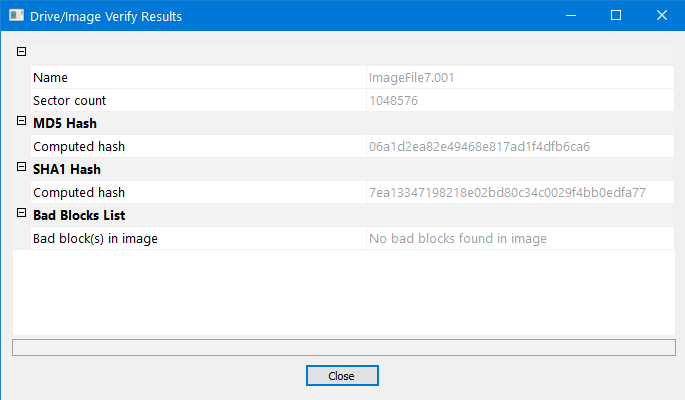
\includegraphics[width=0.7\textwidth]{figures/hash}
  \caption{Image Hash}
  \label{f:image-hash}
\end{figure}

\subsection{EWF/E01 Image Files}
\label{s:task1-part-a-ewf-e01-file}
For this tasks, two different methods and images are being created. To create
the images, the dialog to create images has been opened on \lstinline{FTK Imager}.

\begin{figure}[H]
  \centering
  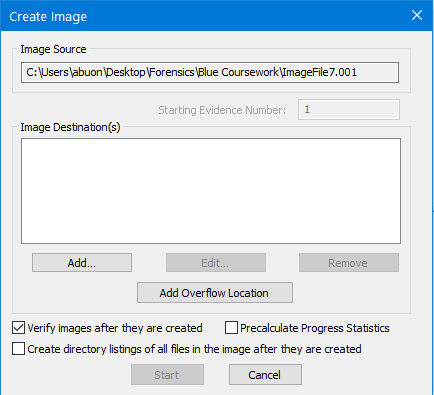
\includegraphics[width=0.6\textwidth]{figures/create-images}
  \caption{Create Images on FTK Imager}
  \label{f:create-images}
\end{figure}

Clicking on \lstinline{Add} will open another dialog that asks for evidence
information.

\begin{figure}[H]
  \centering
  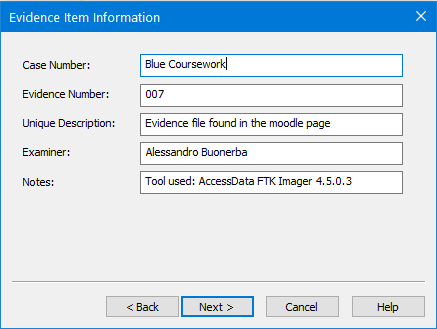
\includegraphics[width=0.6\textwidth]{figures/evidence-information}
  \caption{Evidence Information}
  \label{f:evidence-information}
\end{figure}

The next step is used to selected the image destination, the filename and
various options such as fragmentation and compression.

\begin{figure}[H]
  \centering
  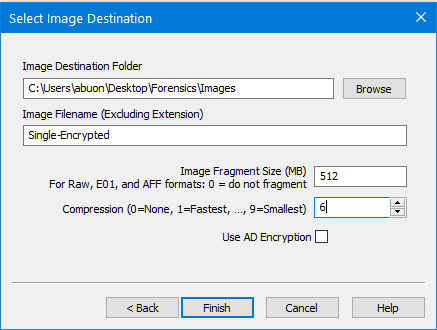
\includegraphics[width=0.6\textwidth]{figures/single-encrypted}
  \caption{Single Encrypted Image}
  \label{f:single-encrypted}
\end{figure}

The figure above represents the first requirements that asks to create a single
E01 image file with enabled compression that in this case is set on 6, while the
figure below represents the splitted version without compression.

\begin{figure}[H]
  \centering
  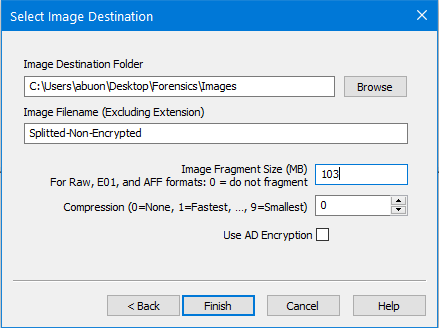
\includegraphics[width=0.6\textwidth]{figures/splitted-no-compression}
  \caption{Fragmented Image without Compression}
  \label{f:splitted-no-compression}
\end{figure}

Since the image to be split is 512mb and the new E01 must be split in 5 files,
the image fragment size has been set dividing the two numbers, resulting in
103mb. After closing the dialog, the previous create image dialog is shown again
with the image destinations and configurations that has been set previously for
the two tasks.

\begin{figure}[H]
  \centering
  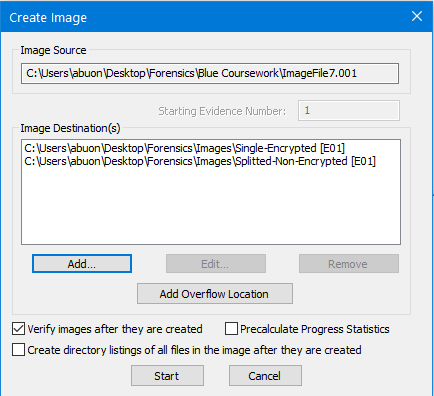
\includegraphics[width=0.6\textwidth]{figures/create-image-start}
  \caption{Create Image Dialog with Images}
  \label{f:create-image-start}
\end{figure}

Clicking on start will initialise the creation of both and at the end of the
process a verify result dialog will pop up with informations on both image
output and their hashes.

\begin{figure}[H]
  \centering
  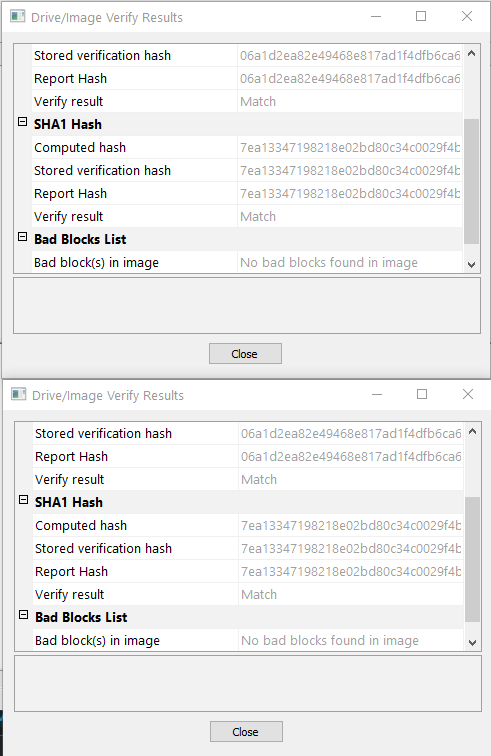
\includegraphics[width=0.5\textwidth]{figures/end-process-hashes}
  \caption{Verify Result Dialog}
  \label{f:end-process-hashes}
\end{figure}

The following image captures the structure of the output files we previously
created. It confirms that the splitted files are indeed 5.

\begin{figure}[H]
  \centering
  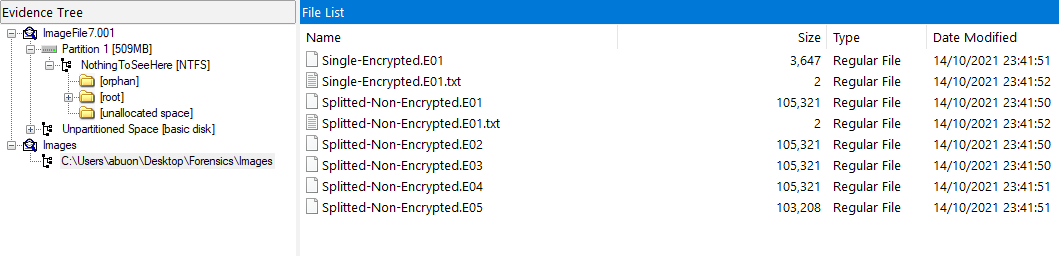
\includegraphics[width=0.8\textwidth]{figures/folder-structure}
  \caption{File Structures}
  \label{f:folder-structure}
\end{figure}

\section{Part B}
\label{s:task1-part-b}
Previously, \lstinline{FTK Imager} has been used to accomplish the tasks, and
the previously screenshots to document the hashes of the images created. To
perform Dual Tool Verification, \lstinline{Autopsy} is also used on this task to
double-check the image hashes. The following screenshots confirm that the hashes
are the same, meaning that nothing has been tempered.

\begin{figure}[H]
  \centering
  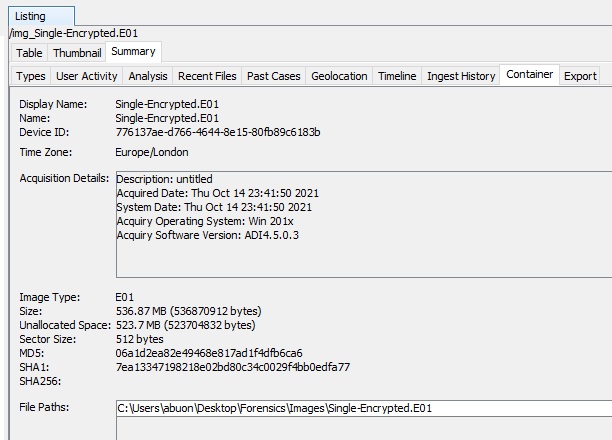
\includegraphics[width=0.7\textwidth]{figures/autopsy-hashes}
  \caption{Autopsy Dual Tool Verification}
  \label{f:autopsy-hashes}
\end{figure}

\newpage
\section{Part C}
\label{s:task1-part-c}
The following would be a description suitable for the members of a jury without
technical knowledge.

\subsection{Write blocker}
\label{s:write-blocker}
A \lstinline{Write blocker} is a small portable device used by investigators to examine USBs
or other removable media without tempering the evidences that are being examined,
preserving authenticity.


  \chapter{Task 2: Search and Seizure}\label{c:Task-2}
  Task 2 Forensics


  \chapter{Task 3: Written Evidence}\label{c:Task-3}
  In this task I will be producing a statement after conducting an individual
analysis on a provided image file. The MG11 statement will be the results of
such analysis with elaboration on evidences and examinations done.
\newline\newline\textbf{Scenario Outline}\newline
You are the duty Digital Forensics Analyst at the Greenwich
Police Hi-Tech Forensics Unit (HTFU). You have received the forensic image file
`Operation Blue 3 - 2021.E01' from the duty Imaging Technician, A\@. Aaron
Adamson, relating to an urgent examination that is required on an exhibit ABL/1.
\newline\newline\textbf{Circumstances}\newline
At approximately 2340hrs on Tuesday the 19th of 2021 DC LITTLE
(4012RG) in company with DC LARGE (1006RG) as part of `Operation Blue 3' stopped
a dark coloured Golf GTi on Glaisher street SE8, for suspicion of distribution
of drugs, in a `Deliveroo for Drugs' type of operation. Two males, James
PRZYBYLOWICZ (DOB 5/1/2001) and Simon VAN DER VALK (DOB 1/5/2000) were present
in the vehicle. VAN DER VALK jumped out of the passenger side of the car, ran to
the edge of the river and threw what appeared to be a small rucksack into the
Thames before LARGE was able to arrest him. A Duty boat was dispatched from
Wapping MPU but was not able to locate the bag. The suspects did not have any
mobile phones on their person. A small removable computer drive (exhibit ABL/1)
was found in the footwell of the passenger side of the vehicle, along with a
lighter and cigarette rolling paper. A Section 18 search of VAN DER VALK's home
address has turned up computer paraphernalia and a laptop bag, but no computer
has been located. VAN DER VALK states that his computer ``broke ages ago'' and
he got rid of it. PRZYBYLOWICZ has made a no comment interview. VAN DER VALK has
stated that he has no knowledge of ABL/1. VAN DER VALK states that he had ``A
little bit of weed'' in his bag, and he threw it in the river because he
panicked, stating that he didn't want to be thrown out of university, as he is
on a student visa. VAN DER VALK has shown student identification documents
showing he studies Business Information Systems at the University of Greenwich.

\section{Evidential Extraction Document}
\label{s:evidential-extraction-document}
\subsection{Notable Files and Documents}
\label{s:evidential-extraction-document-notable-files-and-documents}
The artefact 1 is related to paragraph 26 of the statement dated 06/11/2021.
\begin{figure}[H]
  \centering
  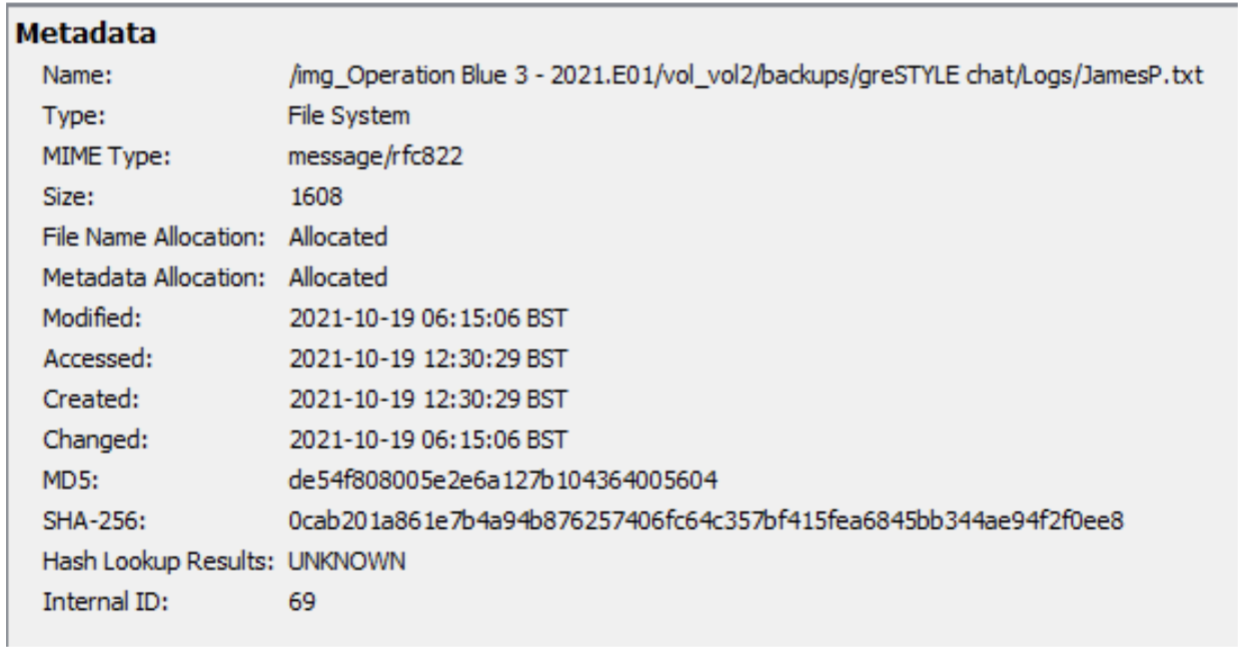
\includegraphics[width=0.8\textwidth]{figures/meta1}
  \caption{Artefact 1: JamesP.txt}
  \label{f:meta1}
\end{figure}
\subsection{Chats and Website}
\label{s:evidential-extraction-document-chats}
The artefact 2 is related to paragraph 20 of the statement dated 06/11/2021.
\begin{figure}[H]
  \centering
  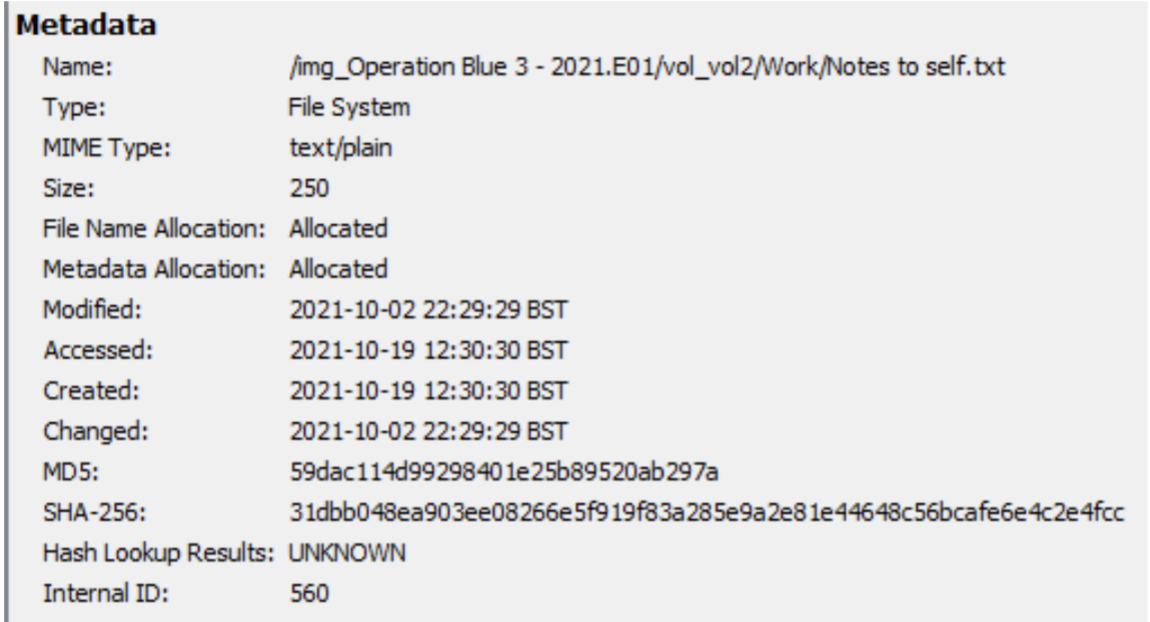
\includegraphics[width=0.8\textwidth]{figures/meta2}
  \caption{Artefact 2: Notes to self.txt}
  \label{f:meta2}
\end{figure}
\newpage
The artefact 3 is related to paragraph 21 of the statement dated 06/11/2021.
\begin{figure}[H]
  \centering
  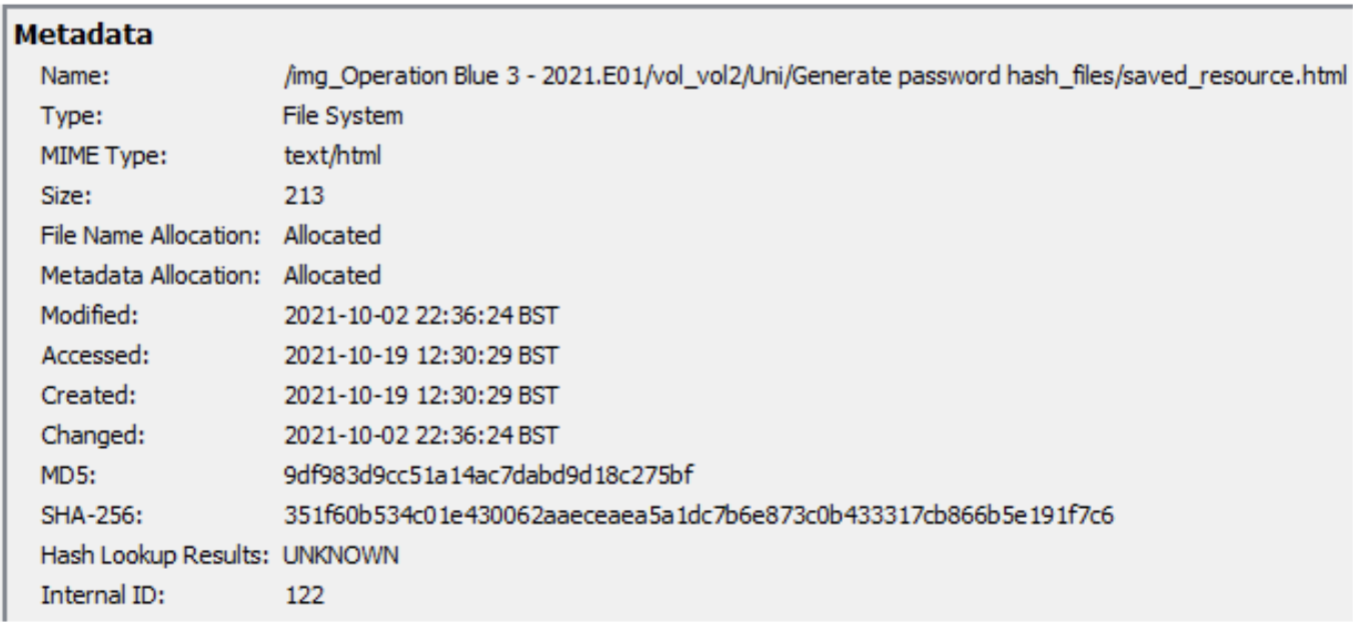
\includegraphics[width=0.8\textwidth]{figures/meta3}
  \caption{Artefact 3: \_resource.html}
  \label{f:meta3}
\end{figure}
The artefact 4 is related to paragraph 21 of the statement dated 06/11/2021.
\begin{figure}[H]
  \centering
  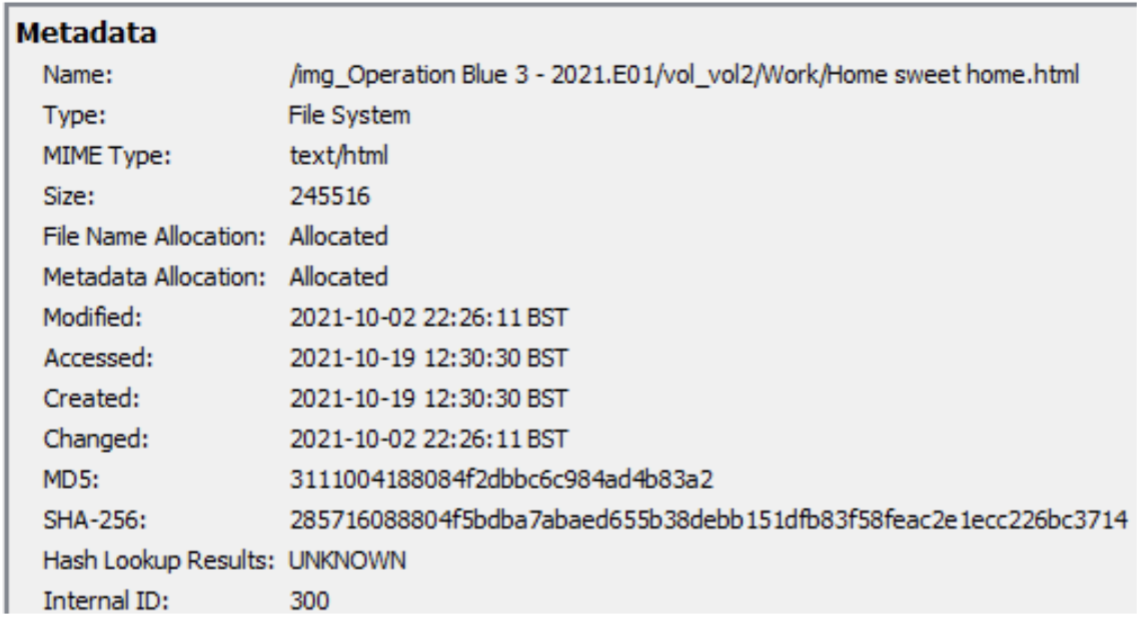
\includegraphics[width=0.8\textwidth]{figures/meta4}
  \caption{Artefact 4: Home sweet home.html}
  \label{f:meta4}
\end{figure}
\newpage
The artefact 5 is related to paragraph 21 of the statement dated 06/11/2021.
\begin{figure}[H]
  \centering
  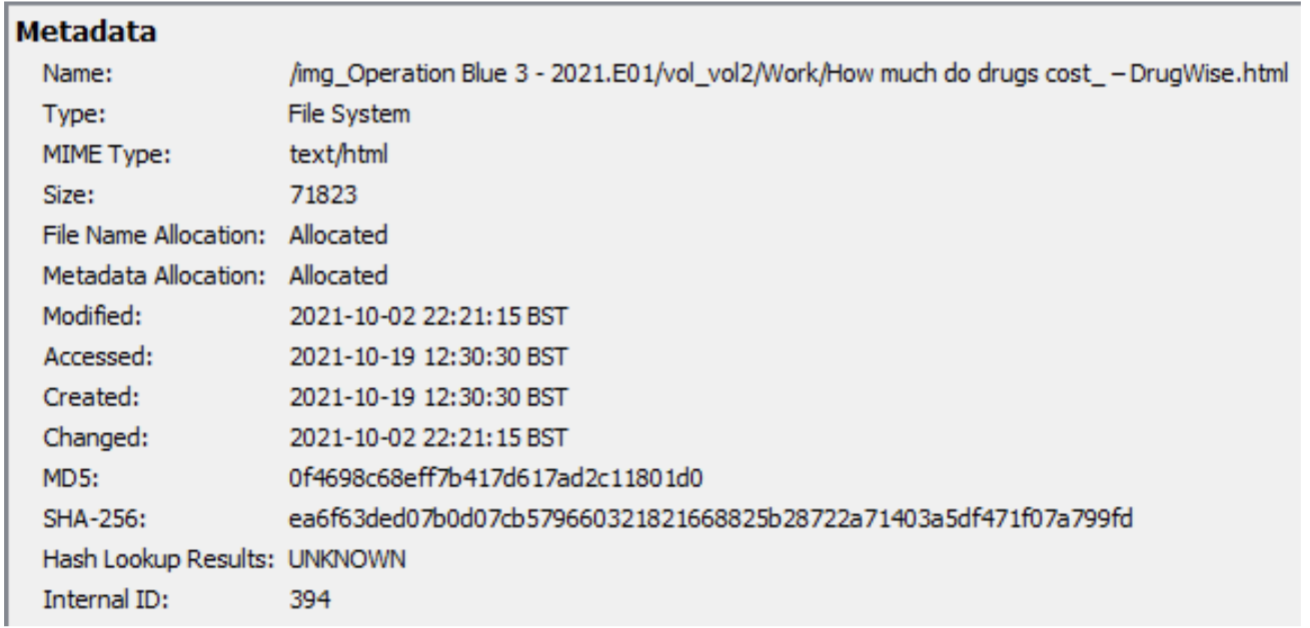
\includegraphics[width=0.8\textwidth]{figures/meta5}
  \caption{Artefact 5: DrugWise.html}
  \label{f:meta5}
\end{figure}
The artefact 6 is related to paragraph 21 of the statement dated 06/11/2021.
\begin{figure}[H]
  \centering
  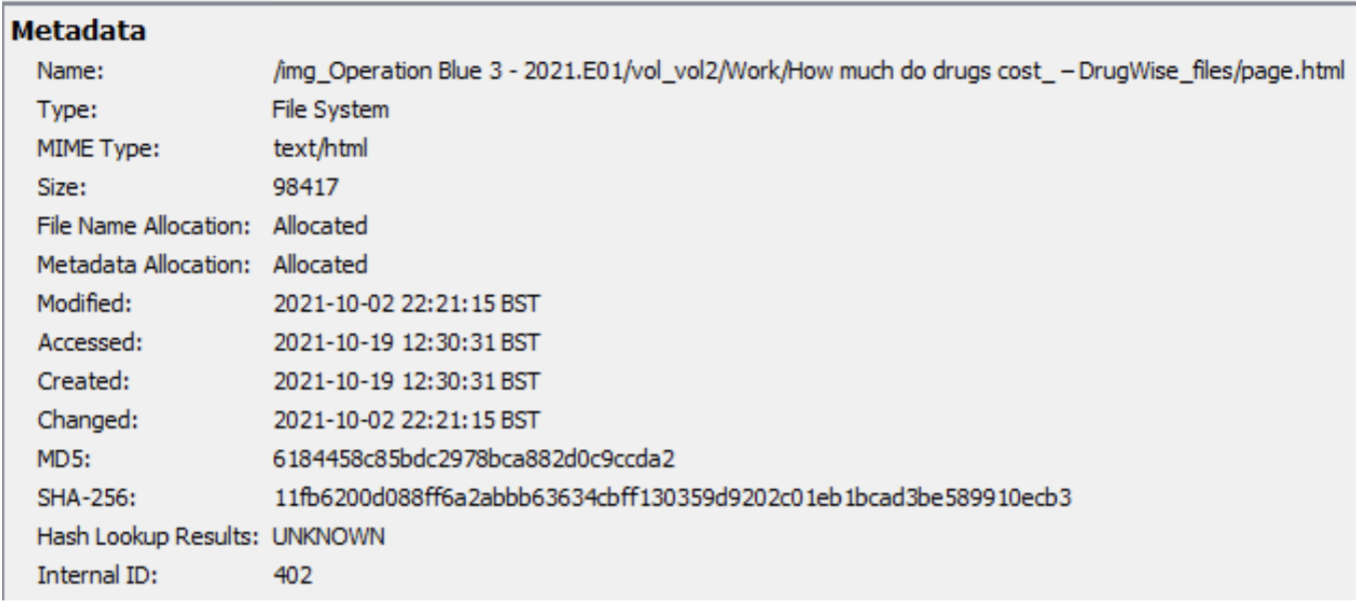
\includegraphics[width=0.8\textwidth]{figures/meta6}
  \caption{Artefact 6: page.html}
  \label{f:meta6}
\end{figure}
\newpage
The artefact 7 is related to paragraph 11 of the statement dated 06/11/2021.
\begin{figure}[H]
  \centering
  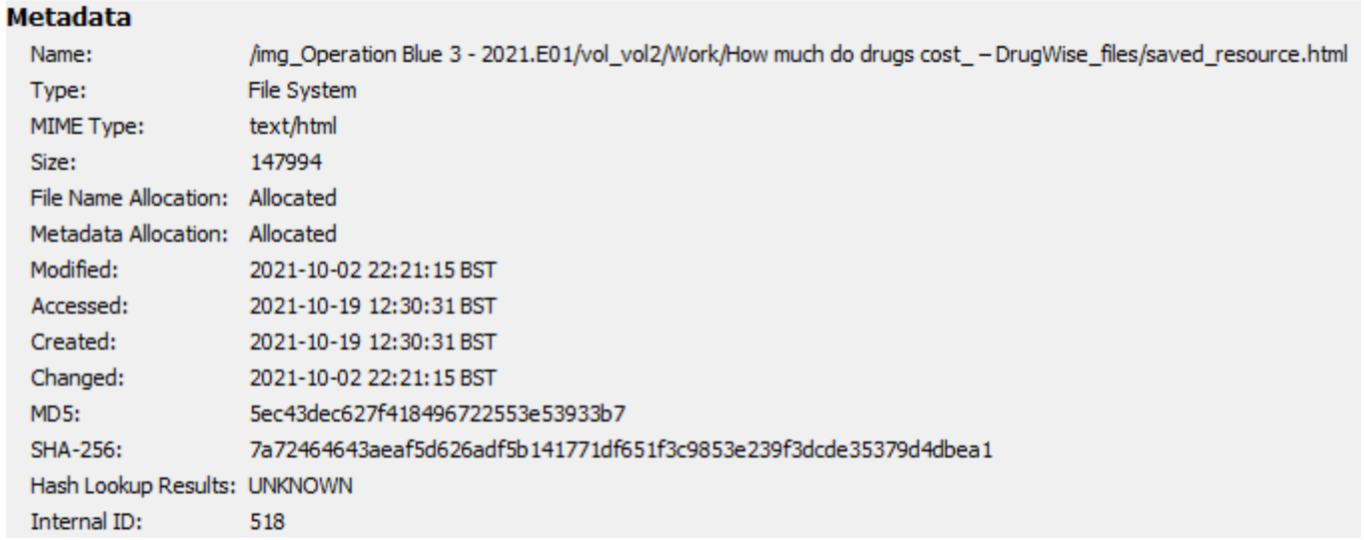
\includegraphics[width=0.8\textwidth]{figures/meta7}
  \caption{Artefact 7: resource.html}
  \label{f:meta7}
\end{figure}
The artefact 8 is related to paragraph 11 of the statement dated 06/11/2021.
\begin{figure}[H]
  \centering
  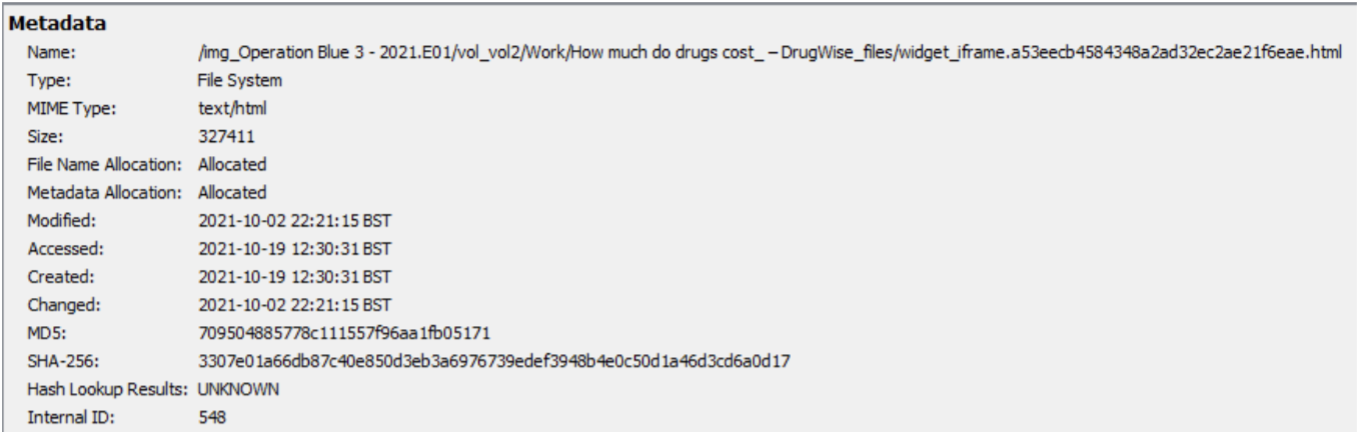
\includegraphics[width=0.8\textwidth]{figures/meta8}
  \caption{Artefact 8: iframe.a53eecb4584348a2ad32ec2ae21f6eae.html}
  \label{f:meta8}
\end{figure}
\newpage
The artefact 9 is related to paragraph 30 of the statement dated 06/11/2021.
\begin{figure}[H]
  \centering
  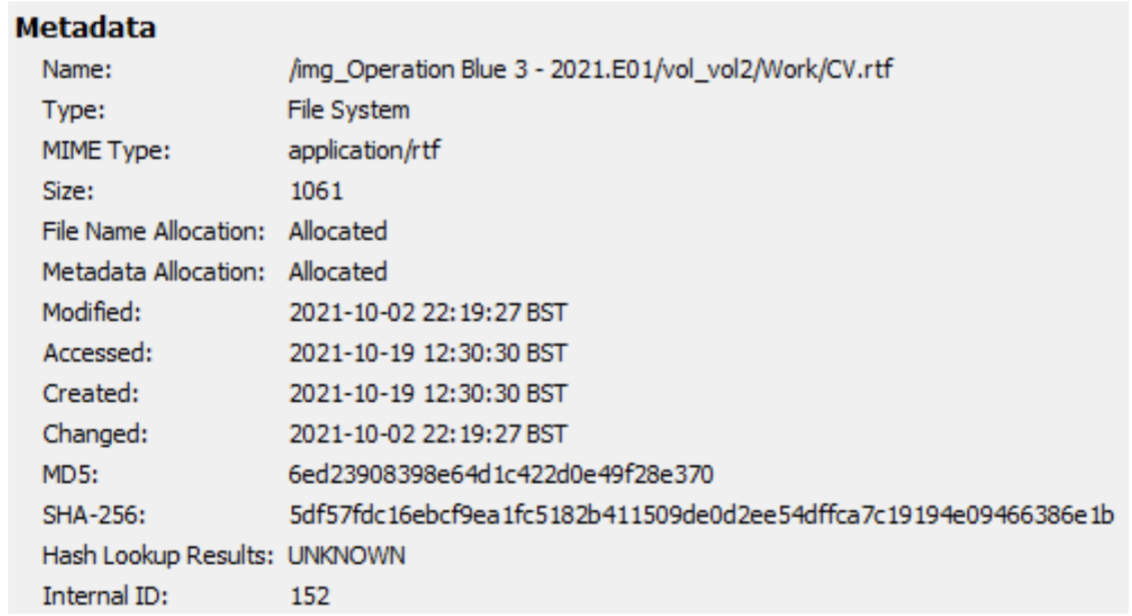
\includegraphics[width=0.8\textwidth]{figures/meta9}
  \caption{Artefact 9: CV.rtf}
  \label{f:meta9}
\end{figure}
The artefact 10 is related to paragraph 26 of the statement dated 06/11/2021.
\begin{figure}[H]
  \centering
  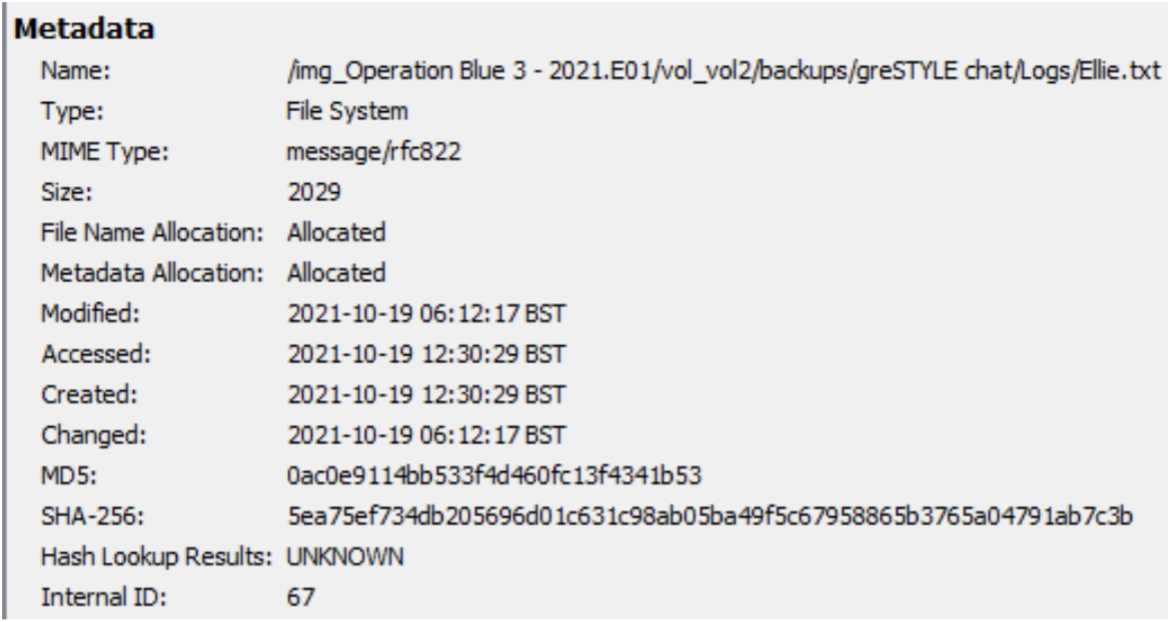
\includegraphics[width=0.8\textwidth]{figures/meta10}
  \caption{Artefact 10: Ellie.txt}
  \label{f:meta10}
\end{figure}

\newpage
\subsection{Drug Material}
The artefact 11 is related to paragraph 23 \& 31 of the statement dated
06/11/2021.

\begin{figure}[H]
  \centering
  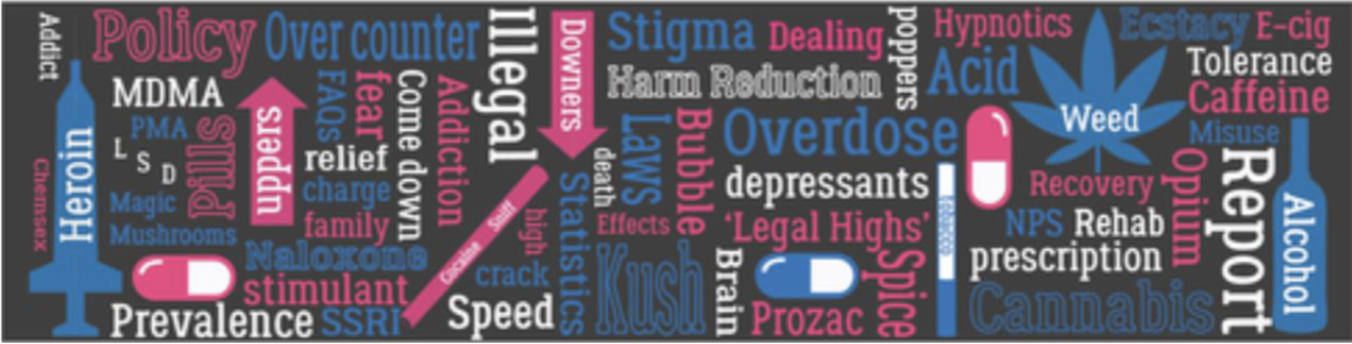
\includegraphics[width=0.8\textwidth]{figures/artefact11}
  \caption{Artefact 11: o.png}
  \label{f:artefact11}
\end{figure}
\begin{figure}[H]
  \centering
  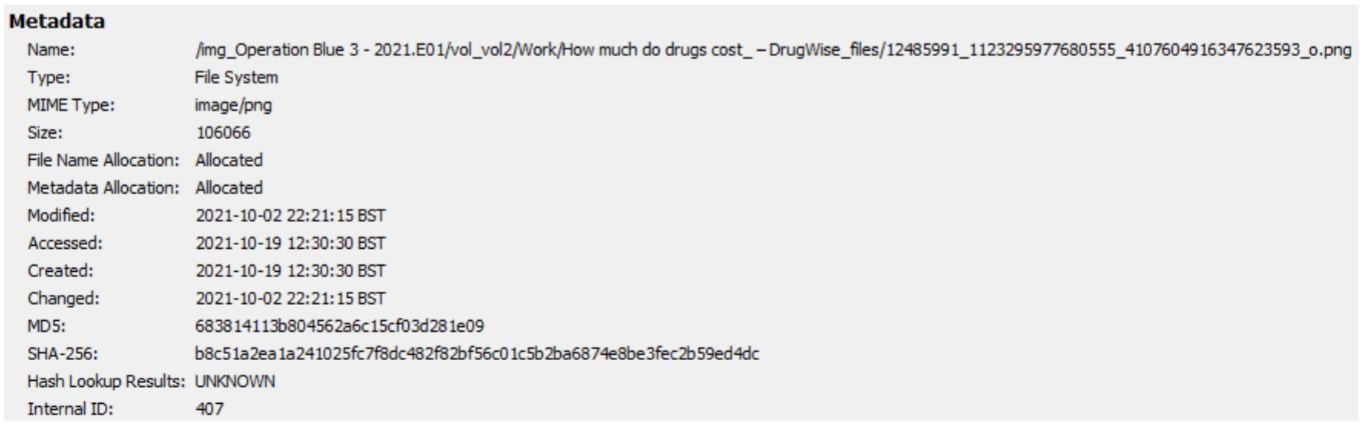
\includegraphics[width=0.8\textwidth]{figures/meta11}
  \caption{Artefact 11: Metadata}
  \label{f:meta11}
\end{figure}
The artefact 12 is related to paragraph 23 \& 31 of the statement dated 06/11/2021.
\begin{figure}[H]
  \centering
  
\includegraphics[width=0.4\textwidth]{figures/artifact12}
  \caption{Artefact 12: n(1).png}
  \label{f:artifact12}
\end{figure}
\begin{figure}[H]
  \centering
  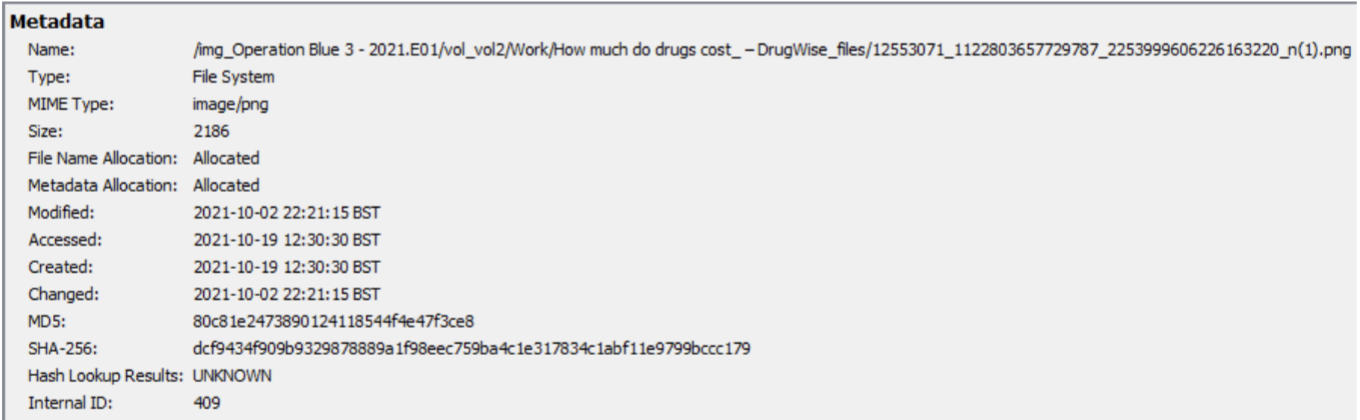
\includegraphics[width=0.8\textwidth]{figures/meta12}
  \caption{Artefact 12: Metadata}
  \label{f:meta12}
\end{figure}
The artefact 13 is related to paragraph 23 \& 31 of the statement dated
06/11/2021.
\begin{figure}[H]
  \centering
  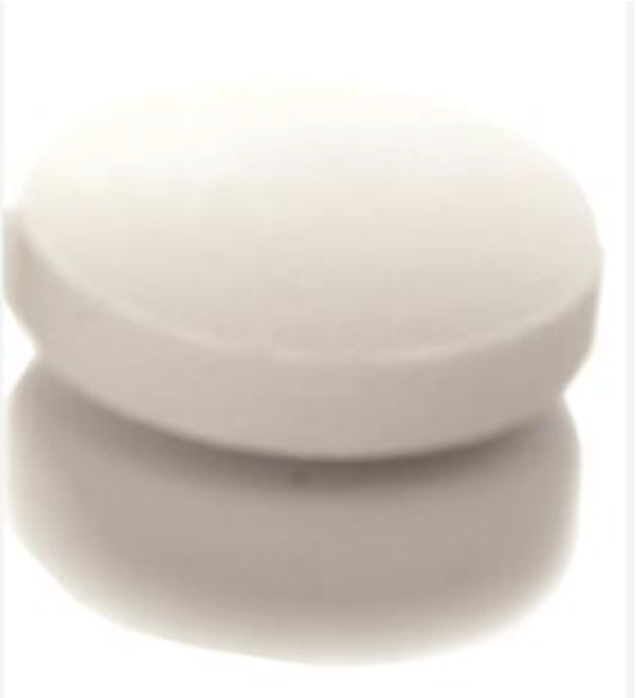
\includegraphics[width=0.4\textwidth]{figures/artefact13}
  \caption{Artefact 13: amphetamines.jpg}
  \label{f:artefact13}
\end{figure}
\begin{figure}[H]
  \centering
  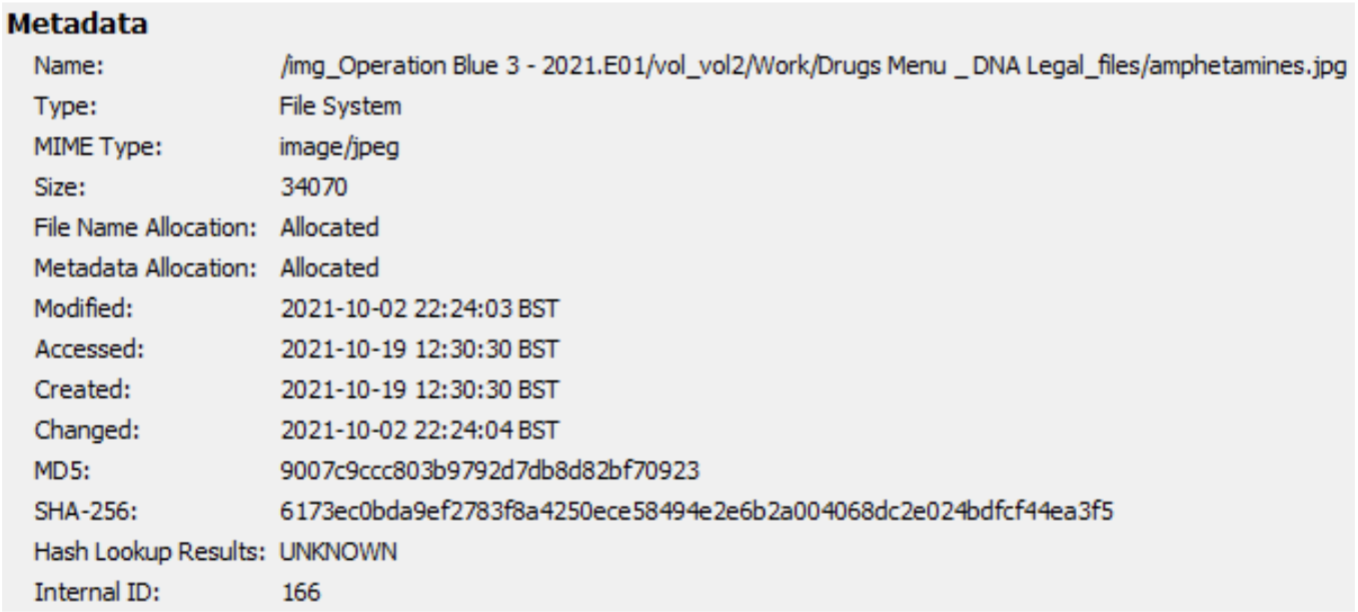
\includegraphics[width=0.8\textwidth]{figures/meta13}
  \caption{Artefact 13: Metadata}
  \label{f:meta13}
\end{figure}
The artefact 14 is related to paragraph 23 \& 31 of the statement dated
06/11/2021.
\begin{figure}[H]
  \centering
  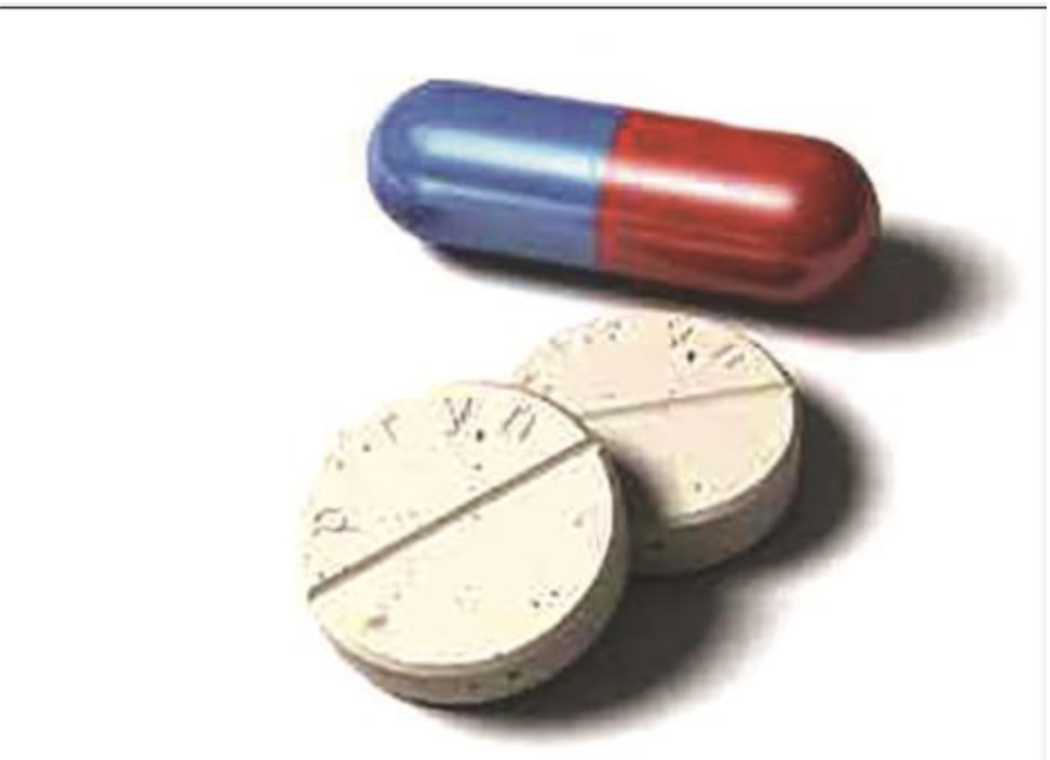
\includegraphics[width=0.4\textwidth]{figures/artefact14}
  \caption{Artefact 14: anabolic-steroids.jpg}
  \label{f:artefact14}
\end{figure}
\begin{figure}[H]
  \centering
  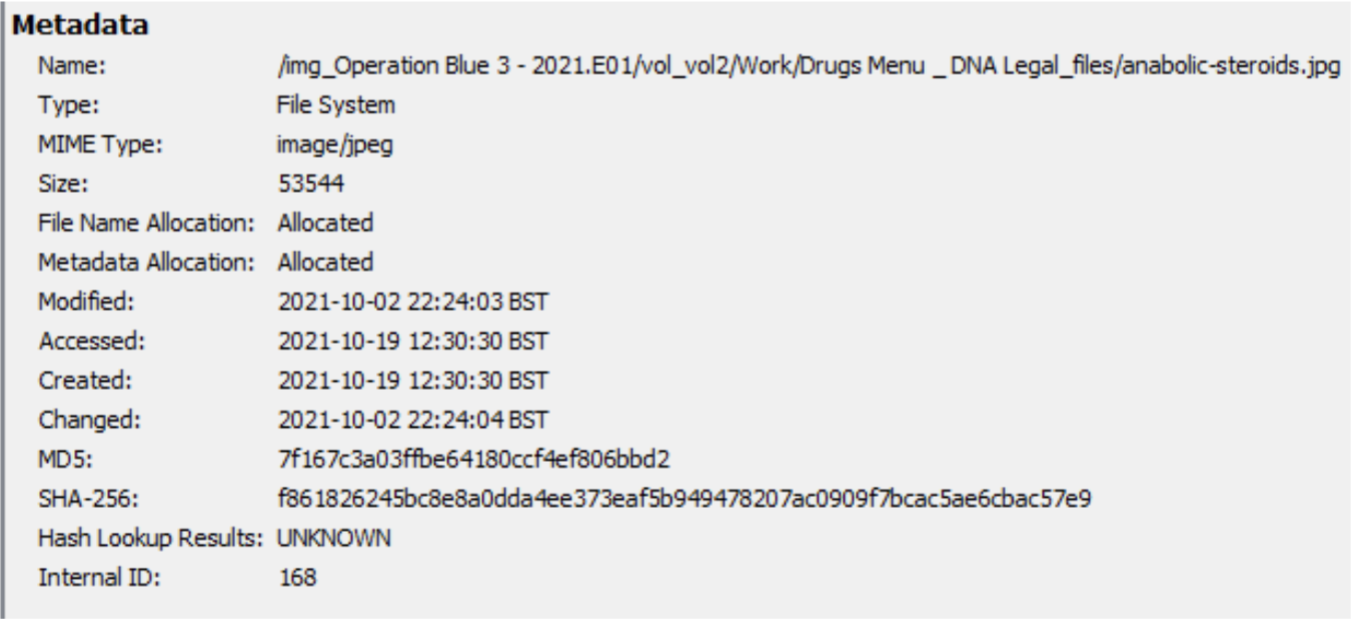
\includegraphics[width=0.8\textwidth]{figures/meta14}
  \caption{Artefact 14: Metadata}
  \label{f:meta14}
\end{figure}
The artefact 15 is related to paragraph 23 \& 31 of the statement dated
06/11/2021.
\begin{figure}[H]
  \centering
  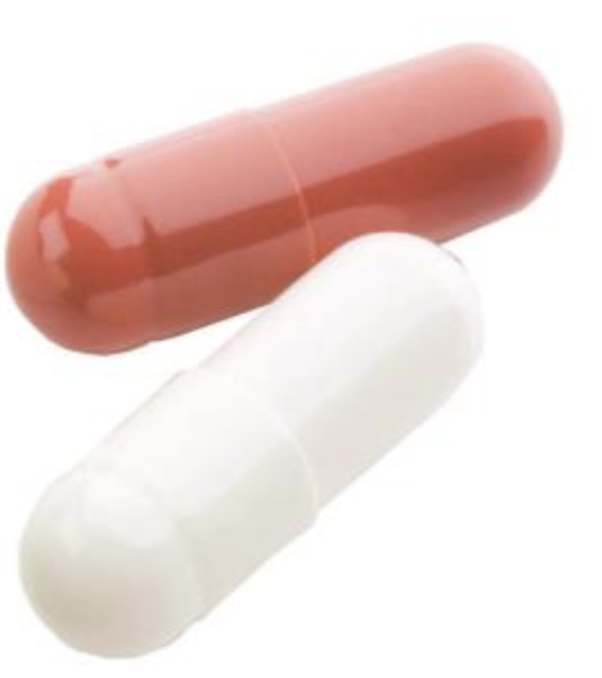
\includegraphics[width=0.4\textwidth]{figures/artefact15}
  \caption{Artefact 15: barbiturates.jpg}
  \label{f:artefact15}
\end{figure}
\begin{figure}[H]
  \centering
  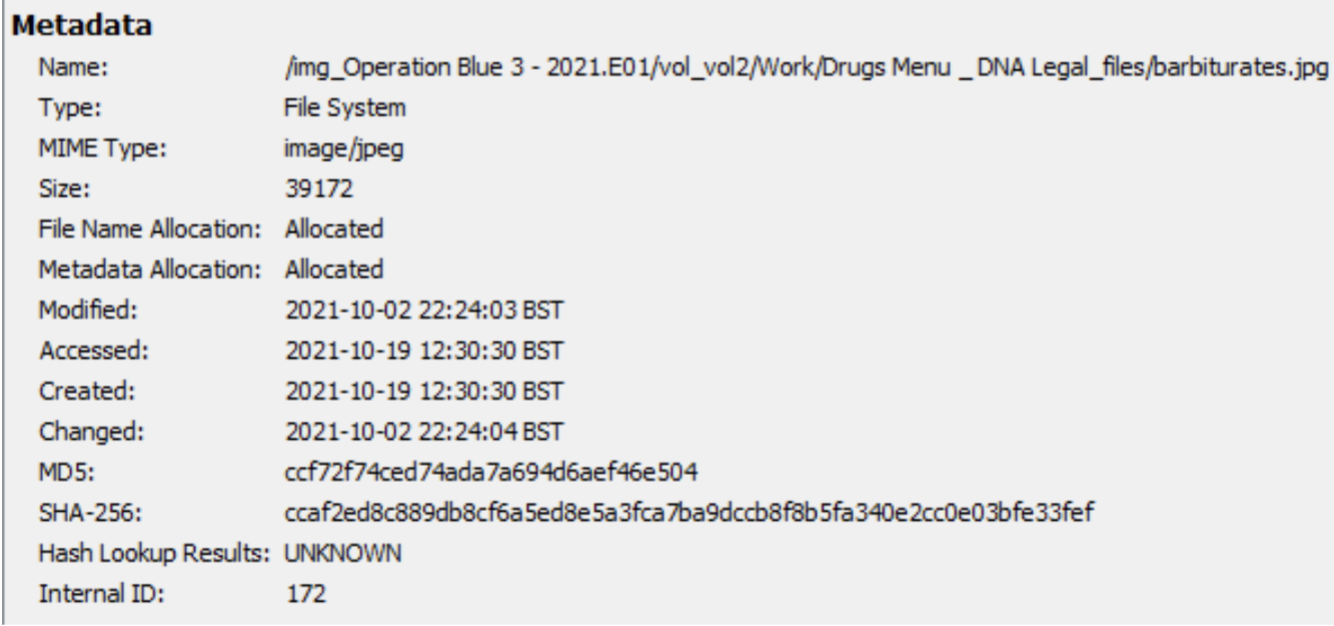
\includegraphics[width=0.8\textwidth]{figures/meta15}
  \caption{Artefact 15: Metadata}
  \label{f:meta15}
\end{figure}
The artefact 16 is related to paragraph 23 \& 31 of the statement dated
06/11/2021.
\begin{figure}[H]
  \centering
  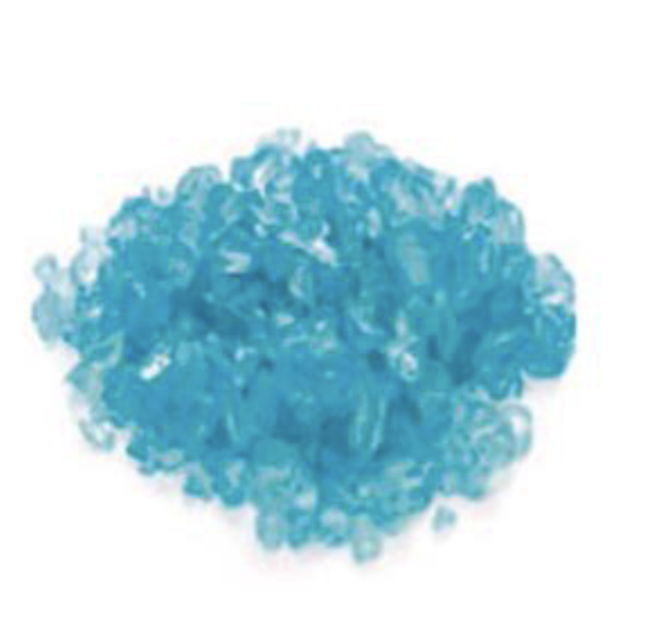
\includegraphics[width=0.4\textwidth]{figures/artefact16}
  \caption{Artefact 16: bath-salts.jpg}
  \label{f:artefact16}
\end{figure}
\begin{figure}[H]
  \centering
  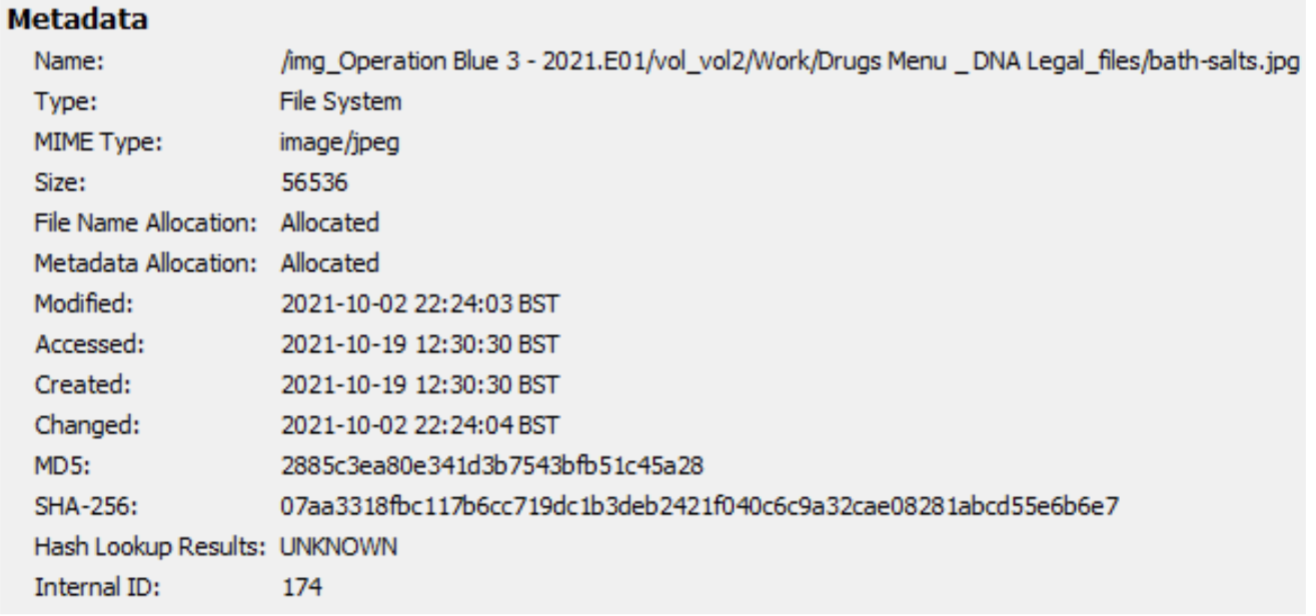
\includegraphics[width=0.8\textwidth]{figures/meta16}
  \caption{Artefact 16: Metadata}
  \label{f:meta16}
\end{figure}
The artefact 17 is related to paragraph 23 \& 31 of the statement dated
06/11/2021.
\begin{figure}[H]
  \centering
  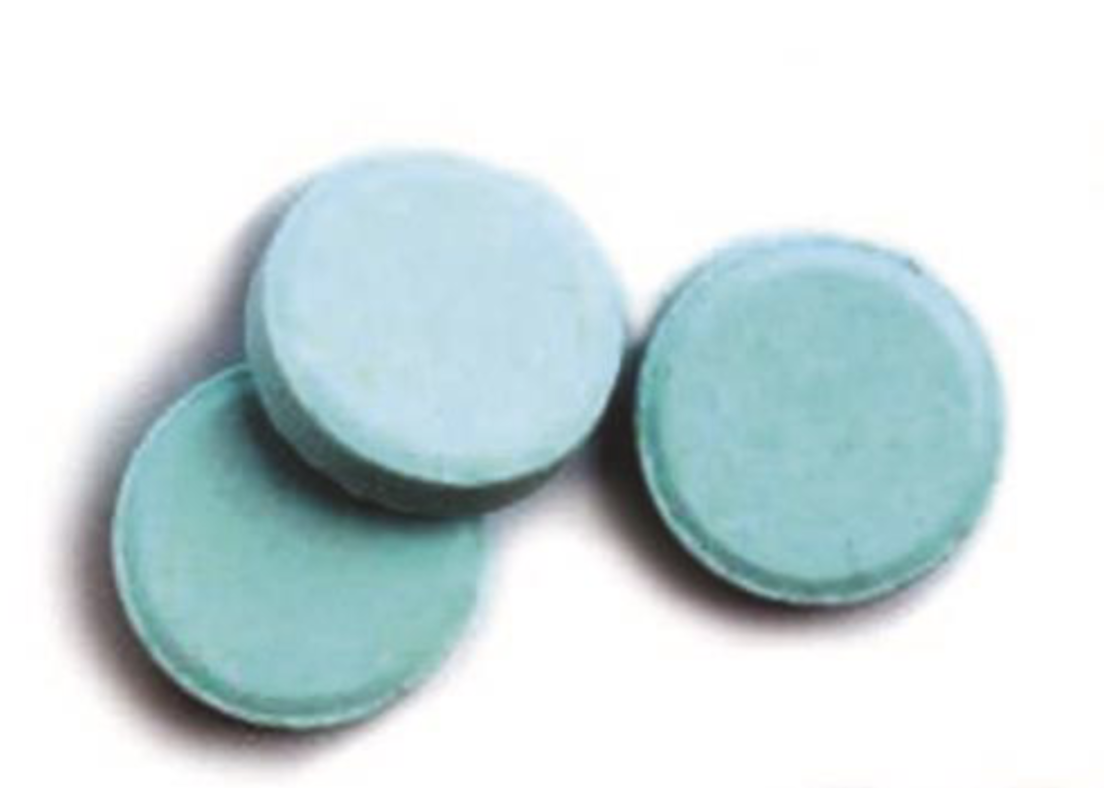
\includegraphics[width=0.4\textwidth]{figures/artefact17}
  \caption{Artefact 17: benzos.jpg}
  \label{f:artefact17}
\end{figure}
\begin{figure}[H]
  \centering
  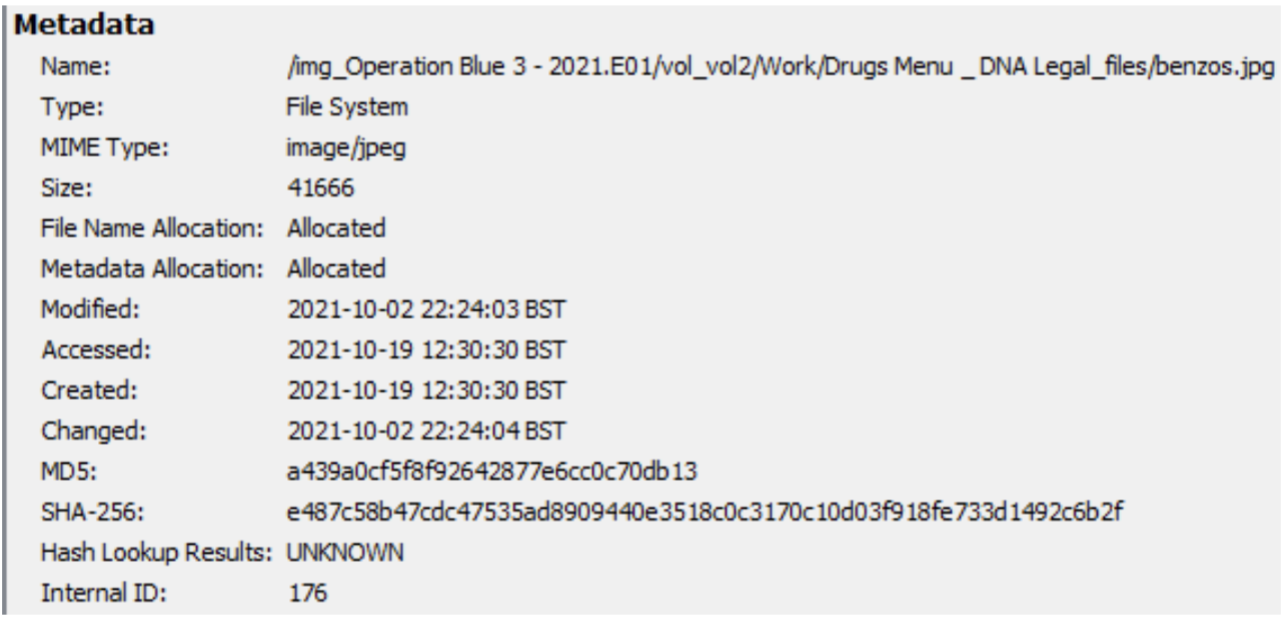
\includegraphics[width=0.8\textwidth]{figures/meta17}
  \caption{Artefact 17: Metadata}
  \label{f:meta17}
\end{figure}
The artefact 18 is related to paragraph 23 \& 31 of the statement dated
06/11/2021
\begin{figure}[H]
  \centering
  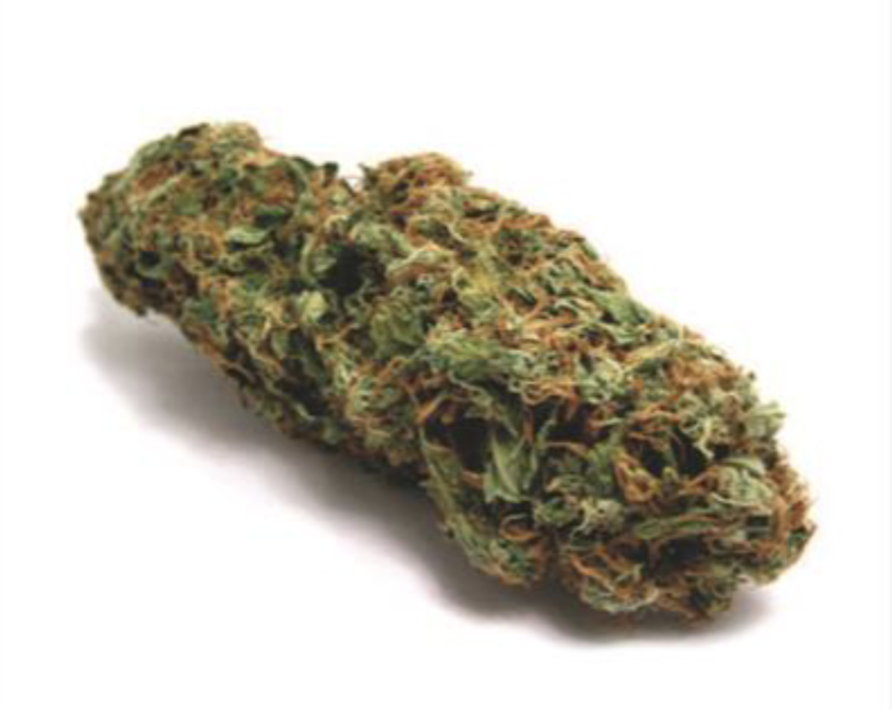
\includegraphics[width=0.4\textwidth]{figures/artefact18}
  \caption{Artefact 18: cannabis.jpg}
  \label{f:artefact18}
\end{figure}
\begin{figure}[H]
  \centering
  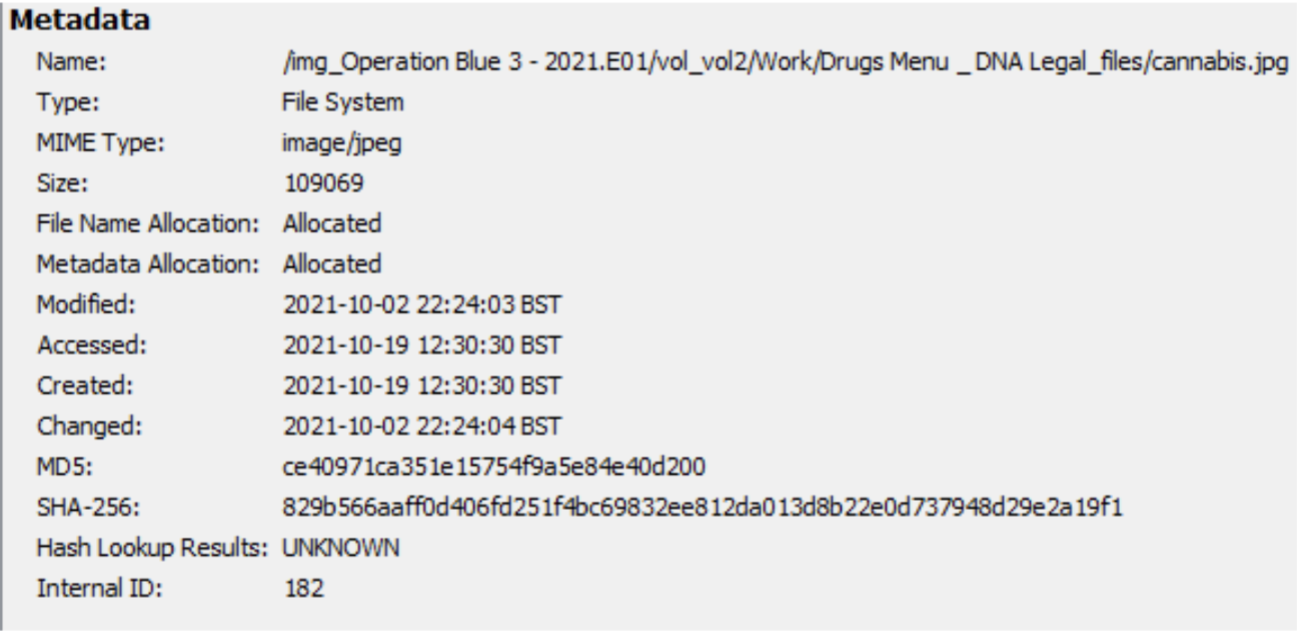
\includegraphics[width=0.8\textwidth]{figures/meta18}
  \caption{Artefact 18: Metadata}
  \label{f:meta18}
\end{figure}
The artefact 19 is related to paragraph 23 \& 31 of the statement dated
06/11/2021
\begin{figure}[H]
  \centering
  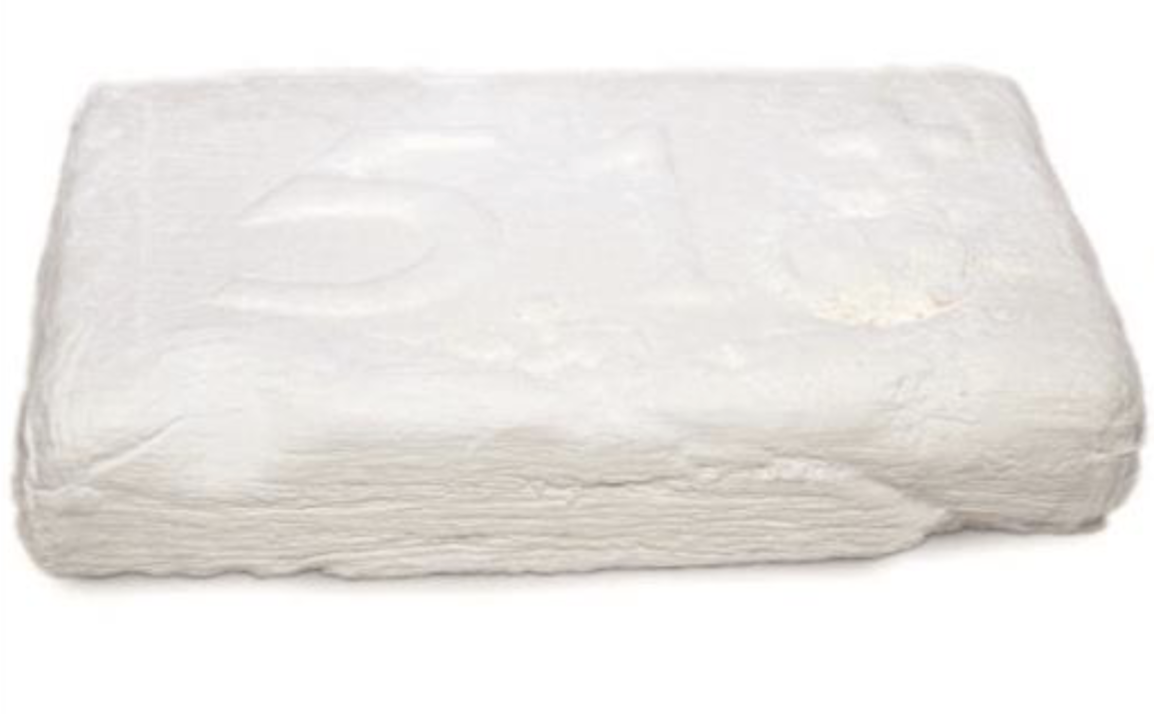
\includegraphics[width=0.6\textwidth]{figures/artefact19}
  \caption{Artefact 19: cocaine-and-crack.jpg}
  \label{f:artefact19}
\end{figure}
\begin{figure}[H]
  \centering
  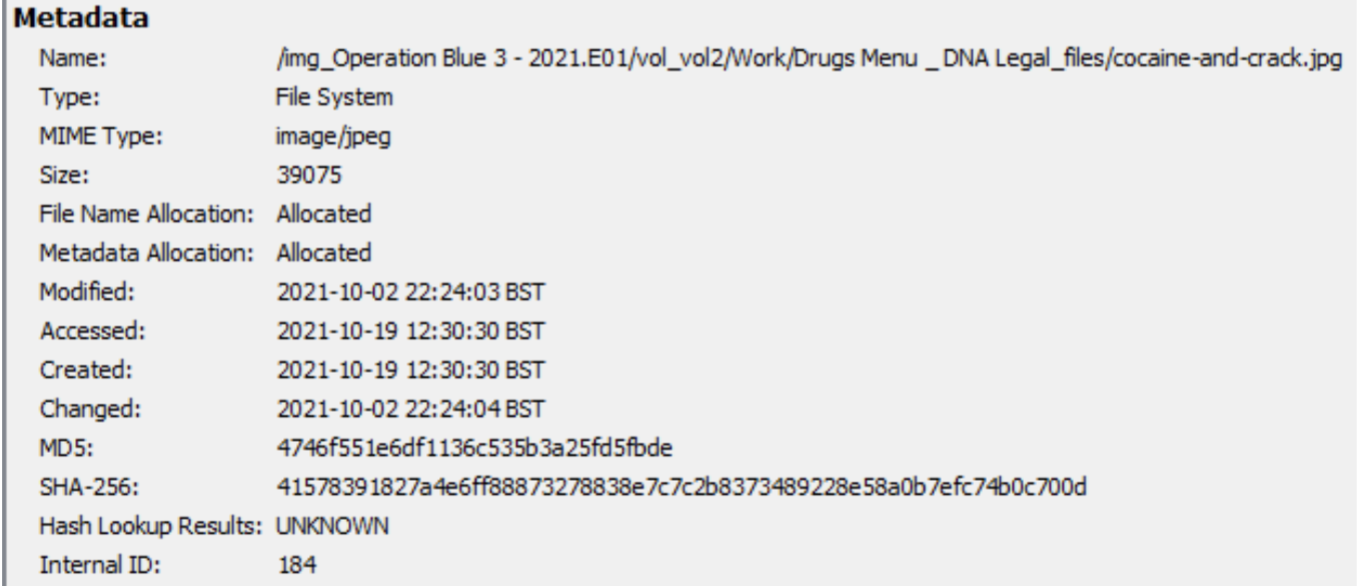
\includegraphics[width=0.8\textwidth]{figures/meta19}
  \caption{Artefact 19: Metadata}
  \label{f:meta19}
\end{figure}
The artefact 20 is related to paragraph 23 \& 31 of the statement
dated 06/11/2021
\begin{figure}[H]
  \centering
  
\includegraphics[width=0.6\textwidth]{figures/artefact20}
  \caption{Artefact 20: dns-drugs-dnslegal.jpg}
  \label{f:artefact20}
\end{figure}
\begin{figure}[H]
  \centering
  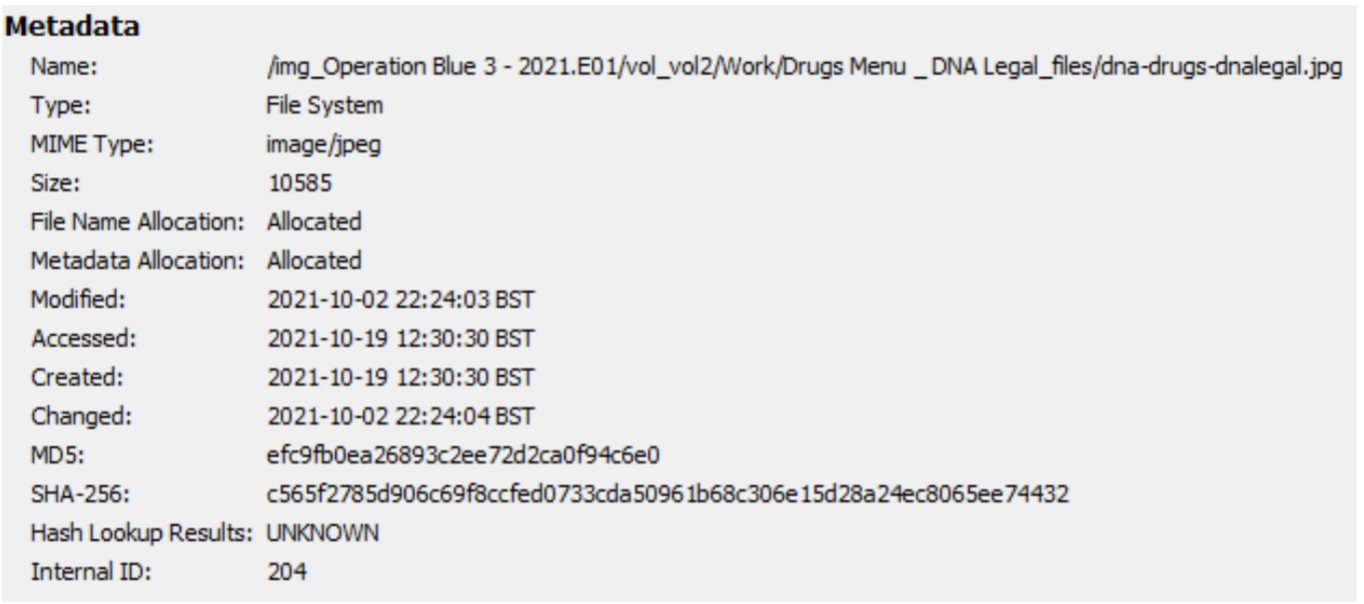
\includegraphics[width=0.8\textwidth]{figures/meta20}
  \caption{Artefact 20: Metadata}
  \label{f:meta20}
\end{figure}
The artefact 21 is related to paragraph 23 \& 31 of the statement
dated 06/11/2021
\begin{figure}[H]
  \centering
  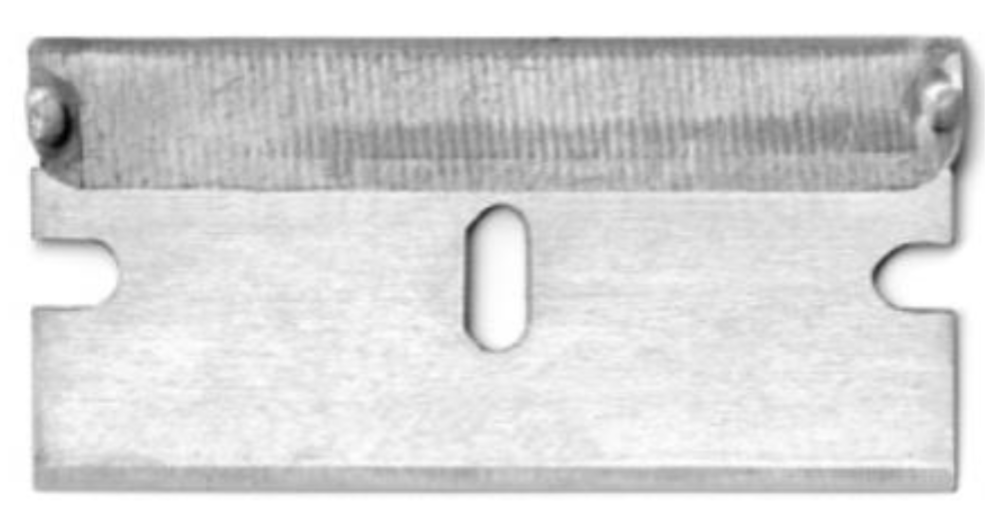
\includegraphics[width=0.4\textwidth]{figures/artefact21}
  \caption{Artefact 21: dna-drugs-razor.jpg}
  \label{f:artefact21}
\end{figure}
\begin{figure}[H]
  \centering
  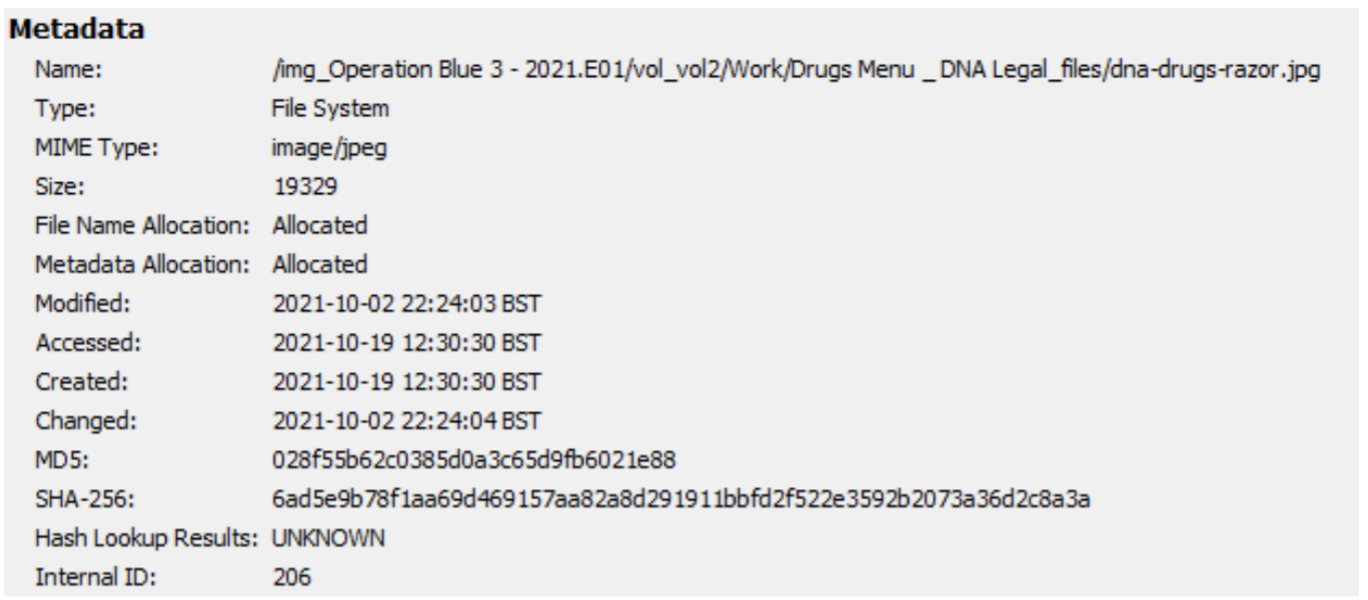
\includegraphics[width=0.8\textwidth]{figures/meta21}
  \caption{Artefact 21: Metadata}
  \label{f:meta21}
\end{figure}
The artefact 22 is related to paragraph 23 \& 31 of the statement dated
06/11/2021
\begin{figure}[H]
  \centering
  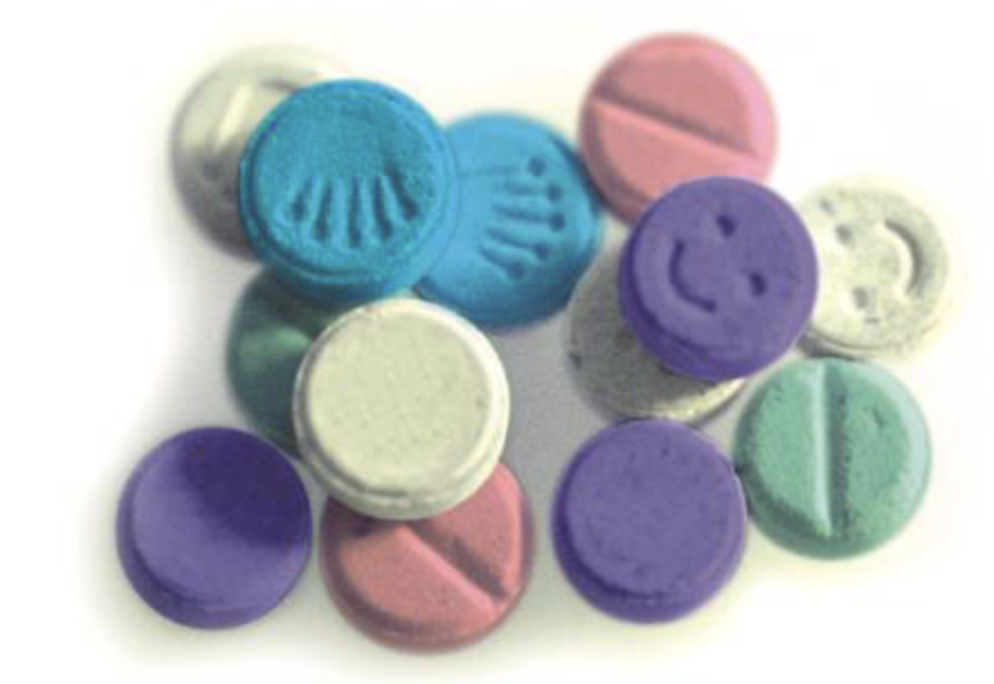
\includegraphics[width=0.4\textwidth]{figures/artefact22}
  \caption{Artefact 22: ecstasy.jpg}
  \label{f:artefact22}
\end{figure}
\begin{figure}[H]
  \centering
  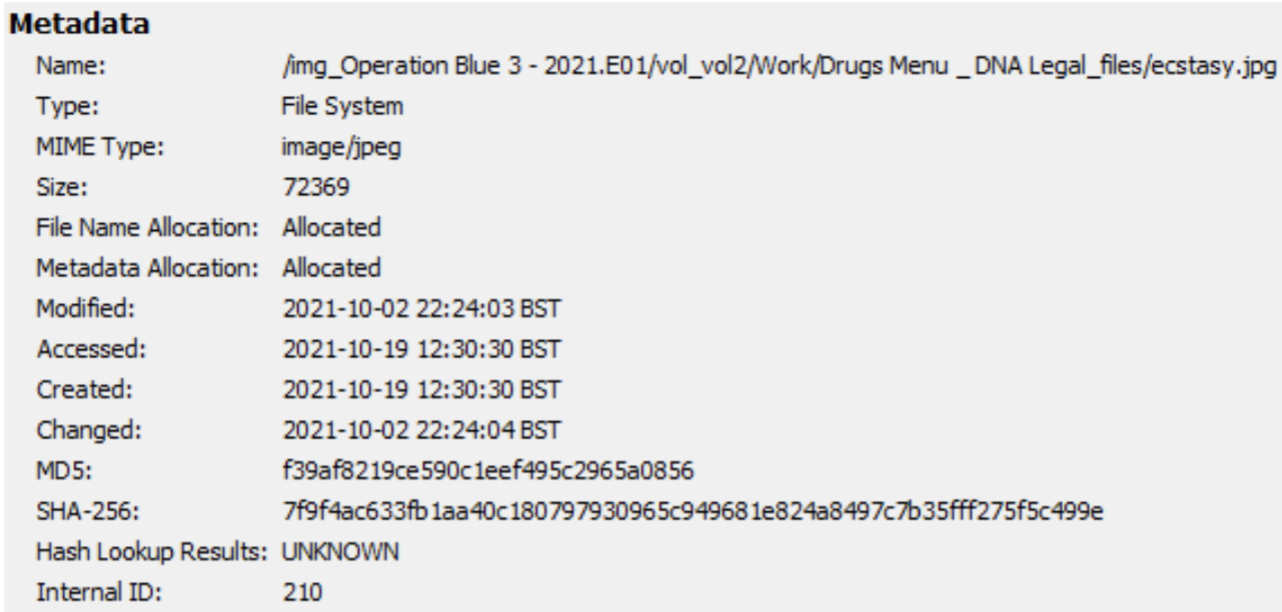
\includegraphics[width=0.8\textwidth]{figures/meta22}
  \caption{Artefact 22: Metadata}
  \label{f:meta22}
\end{figure}
The artefact 23 is related to paragraph 23 \& 31 of the statement
dated 06/11/2021
\begin{figure}[H]
  \centering
  
\includegraphics[width=0.3\textwidth]{figures/artefact23}
  \caption{Artefact 23: ketamine.jpg}
  \label{f:artefact23}
\end{figure}
\begin{figure}[H]
  \centering
  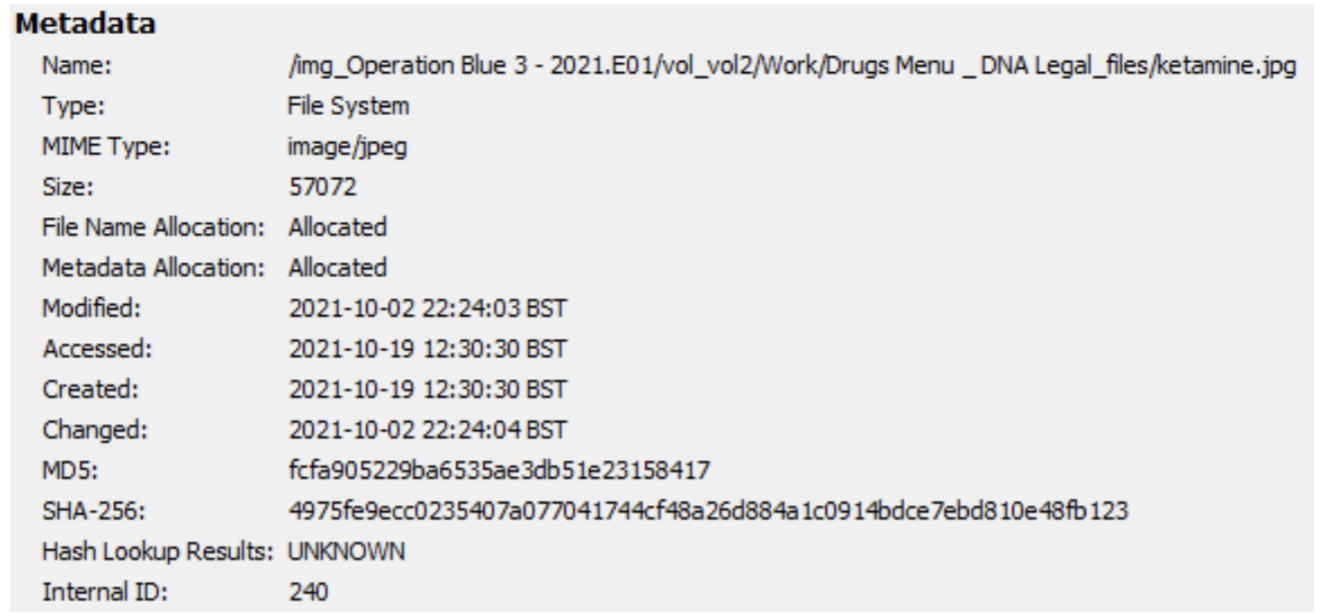
\includegraphics[width=0.8\textwidth]{figures/meta23}
  \caption{Artefact 23: Metadata}
  \label{f:meta23}
\end{figure}
The artefact 24 is related to paragraph 23 \& 31 of the statement dated
06/11/2021
\begin{figure}[H]
  \centering
  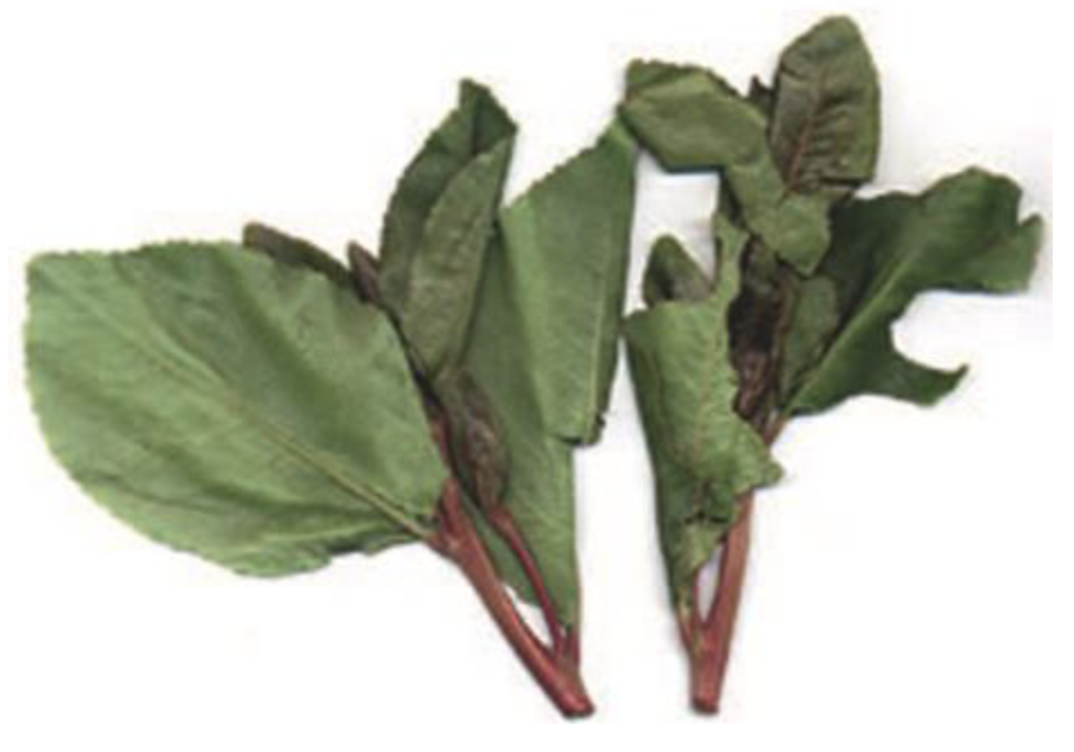
\includegraphics[width=0.4\textwidth]{figures/artefact24}
  \caption{Artefact 24: khat.jpg}
  \label{f:artefact24}
\end{figure}
\begin{figure}[H]
  \centering
  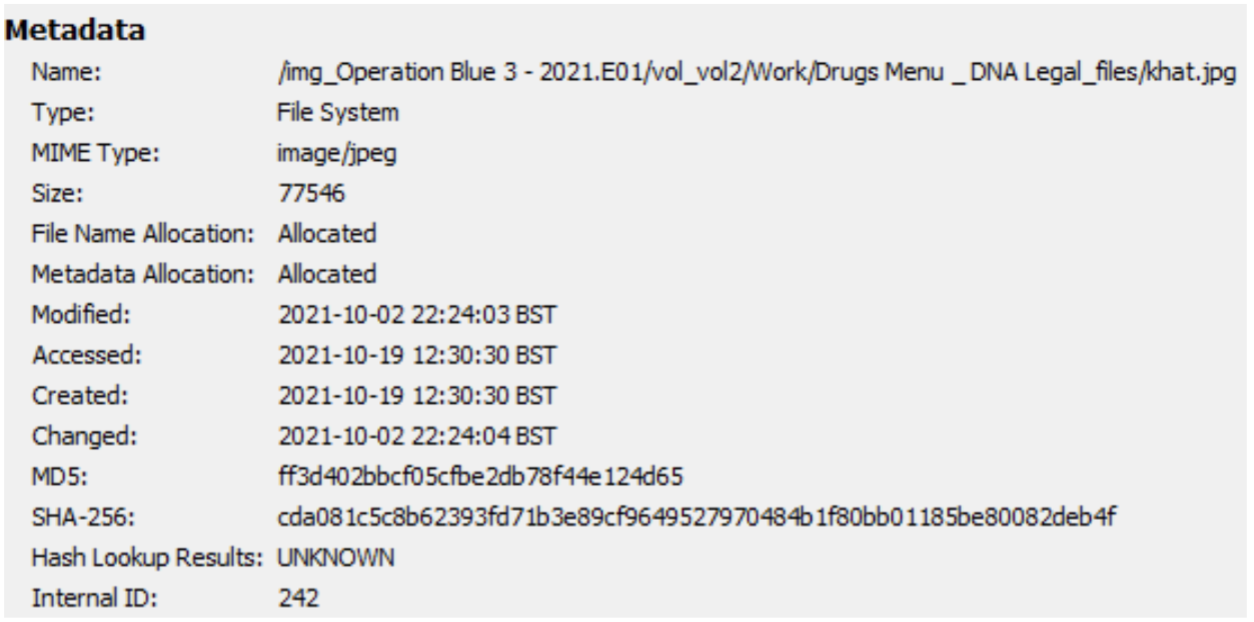
\includegraphics[width=0.8\textwidth]{figures/meta24}
  \caption{Artefact 24: Metadata}
  \label{f:meta24}
\end{figure}
The artefact 25 is related to paragraph 23 \& 31 of the statement
dated 06/11/2021
\begin{figure}[H]
  \centering
  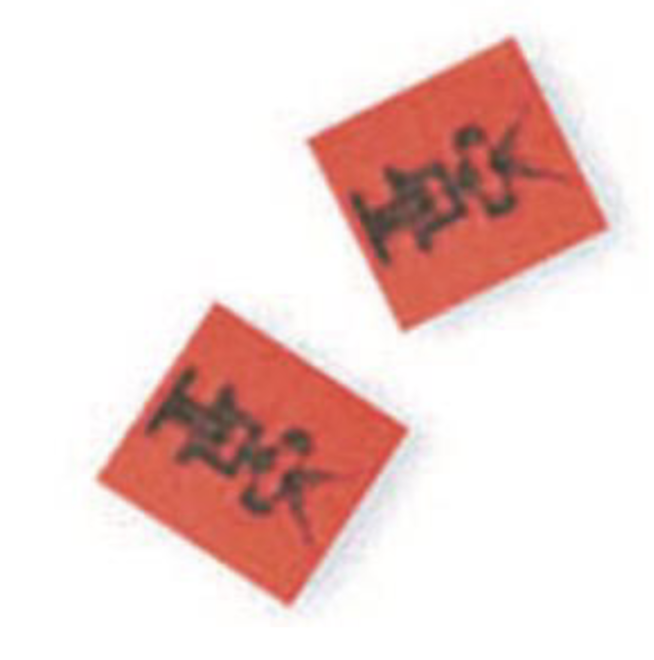
\includegraphics[width=0.4\textwidth]{figures/artefact25}
  \caption{Artefact 25: lsd.jpg}
  \label{f:artefact25}
\end{figure}
\begin{figure}[H]
  \centering
  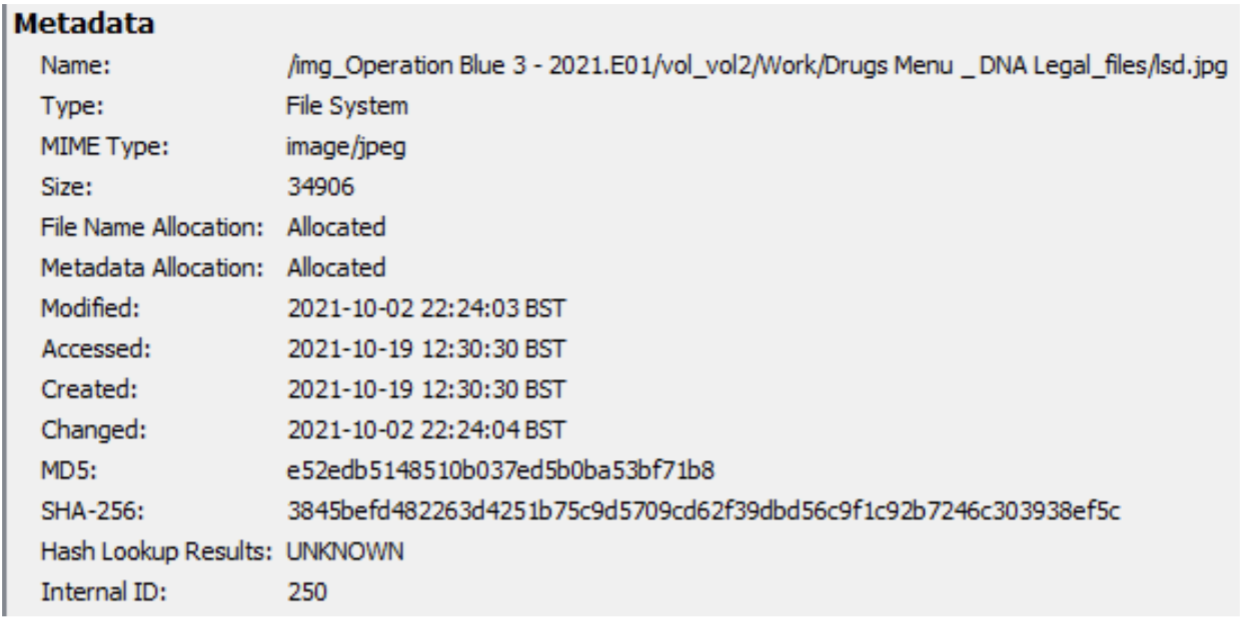
\includegraphics[width=0.8\textwidth]{figures/meta25}
  \caption{Artefact 25: Metadata}
  \label{f:meta25}
\end{figure}
The artefact 26 is related to paragraph 23 \& 31 of the statement
dated 06/11/2021
\begin{figure}[H]
  \centering
  \includegraphics[width=0.4\textwidth]{figures/artefact26}
  \caption{Artefact 26: mephedrone.jpg}
  \label{f:artefact26}
\end{figure}
\begin{figure}[H]
  \centering
  \includegraphics[width=0.8\textwidth]{figures/meta26}
  \caption{Artefact 26: Metadata}
  \label{f:meta26}
\end{figure}
The artefact 27 is related to paragraph 23 \& 31 of the statement
dated 06/11/2021.
\begin{figure}[H]
  \centering
  \includegraphics[width=0.4\textwidth]{figures/artefact27}
  \caption{Artefact 27: methodone.jpg}
  \label{f:artefact27}
\end{figure}
\begin{figure}[H]
  \centering
  \includegraphics[width=0.8\textwidth]{figures/meta27}
  \caption{Artefact 27: Metadata}
  \label{f:meta27}
\end{figure}
The artefact 28 is related to paragraph 23 \& 31 of the statement
dated 06/11/2021.
\begin{figure}[H]
  \centering
  \includegraphics[width=0.4\textwidth]{figures/artefact28}
  \caption{Artefact 28: narcotics.jpg}
  \label{f:artefact28}
\end{figure}
\begin{figure}[H]
  \centering
  \includegraphics[width=0.8\textwidth]{figures/meta28}
  \caption{Artefact 28: Metadata}
  \label{f:meta28}
\end{figure}
The artefact 29 is related to paragraph 23 \& 31 of the statement
dated 06/11/2021.
\begin{figure}[H]
  \centering
  \includegraphics[width=0.4\textwidth]{figures/artefact29}
  \caption{Artefact 29: opiates-heroin.jpg}
  \label{f:artefact29}
\end{figure}
\begin{figure}[H]
  \centering
  \includegraphics[width=0.8\textwidth]{figures/meta29}
  \caption{Artefact 29: Metadata}
  \label{f:meta29}
\end{figure}
The artefact 30 is related to paragraph 23 \& 31 of the statement
dated 06/11/2021.
\begin{figure}[H]
  \centering
  \includegraphics[width=0.4\textwidth]{figures/artefact30}
  \caption{Artefact 30: razor.png}
  \label{f:artefact30}
\end{figure}
\begin{figure}[H]
  \centering
  \includegraphics[width=0.8\textwidth]{figures/meta30}
  \caption{Artefact 30: Metadata}
  \label{f:meta30}
\end{figure}
The artefact 31 is related to paragraph 23 \& 31 of the statement
dated 06/11/2021.
\begin{figure}[H]
  \centering
  \includegraphics[width=0.4\textwidth]{figures/artefact31}
  \caption{Artefact 31: spice-drug.jpg}
  \label{f:artefact31}
\end{figure}
\begin{figure}[H]
  \centering
  \includegraphics[width=0.8\textwidth]{figures/meta31}
  \caption{Artefact 31: Metadata}
  \label{f:meta31}
\end{figure}
The artefact 32 is related to paragraph 23 \& 31 of the statement
dated 06/11/2021.
\begin{figure}[H]
  \centering
  \includegraphics[width=0.4\textwidth]{figures/artefact32}
  \caption{Artefact 32: \_image(1).php}
  \label{f:artefact32}
\end{figure}
\begin{figure}[H]
  \centering
  \includegraphics[width=0.8\textwidth]{figures/meta32}
  \caption{Artefact 32: Metadata}
  \label{f:meta32}
\end{figure}
The artefact 33 is related to paragraph 23 \& 31 of the statement
dated 06/11/2021.
\begin{figure}[H]
  \centering
  \includegraphics[width=0.4\textwidth]{figures/artefact33}
  \caption{Artefact 33: \_image(2).php}
  \label{f:artefact33}
\end{figure}
\begin{figure}[H]
  \centering
  \includegraphics[width=0.8\textwidth]{figures/meta33}
  \caption{Artefact 33: Metadata}
  \label{f:meta33}
\end{figure}
The artefact 34 is related to paragraph 23 \& 31 of the statement
dated 06/11/2021.
\begin{figure}[H]
  \centering
  \includegraphics[width=0.4\textwidth]{figures/artefact34}
  \caption{Artefact 34: safe-image.php}
  \label{f:artefact34}
\end{figure}
\begin{figure}[H]
  \centering
  \includegraphics[width=0.8\textwidth]{figures/meta34}
  \caption{Artefact 34: Metadata}
  \label{f:meta34}
\end{figure}
The artefact 35 is related to paragraph 23 \& 31 of the statement
dated 06/11/2021.
\begin{figure}[H]
  \centering
  \includegraphics[width=0.4\textwidth]{figures/artefact35}
  \caption{Artefact 35: Webp.net-resizeimage-85.jpg}
  \label{f:artefact35}
\end{figure}
\begin{figure}[H]
  \centering
  \includegraphics[width=0.8\textwidth]{figures/meta35}
  \caption{Artefact 35: Metadata}
  \label{f:meta35}
\end{figure}

\section{Indecent and Pornographic Material}
\label{s:pornographic}
The artefact 36 is related to paragraph 24 \& 32 of the statement
dated 06/11/2021.
\begin{figure}[H]
  \centering
  \includegraphics[width=0.4\textwidth]{figures/artefact36}
  \caption{Artefact 36: blondie.jpg}
  \label{f:artefact36}
\end{figure}
\begin{figure}[H]
  \centering
  \includegraphics[width=0.8\textwidth]{figures/meta36}
  \caption{Artefact 36: Metadata}
  \label{f:meta36}
\end{figure}
The artefact 37 is related to paragraph 24 \& 32 of the statement
dated 06/11/2021.
\begin{figure}[H]
  \centering
  \includegraphics[width=0.4\textwidth]{figures/artefact37}
  \caption{Artefact 37: cosplay.jpg}
  \label{f:artefact37}
\end{figure}
\begin{figure}[H]
  \centering
  \includegraphics[width=0.8\textwidth]{figures/meta37}
  \caption{Artefact 37: Metadata}
  \label{f:meta37}
\end{figure}
The artefact 38 is related to paragraph 24 \& 32 of the statement
dated 06/11/2021.
\begin{figure}[H]
  \centering
  \includegraphics[width=0.4\textwidth]{figures/artefact38}
  \caption{Artefact 38: lil asian.jpg}
  \label{f:artefact38}
\end{figure}
\begin{figure}[H]
  \centering
  \includegraphics[width=0.8\textwidth]{figures/meta38}
  \caption{Artefact 38: Metadata}
  \label{f:meta38}
\end{figure}
The artefact 39 is related to paragraph 24 \& 32 of the statement
dated 06/11/2021.
\begin{figure}[H]
  \centering
  \includegraphics[width=0.4\textwidth]{figures/artefact39}
  \caption{Artefact 39: yay retro big hair.jpg}
  \label{f:artefact39}
\end{figure}
\begin{figure}[H]
  \centering
  \includegraphics[width=0.8\textwidth]{figures/meta39}
  \caption{Artefact 39: Metadata}
  \label{f:meta39}
\end{figure}

\section{Pornographic Material}
\label{s:pornographic2}
The artefact 40 is related to paragraph 25 of the statement dated 06/11/2021.
\begin{figure}[H]
  \centering
  \includegraphics[width=0.4\textwidth]{figures/artefact40}
  \caption{Artefact 40: Elizabeth Olson lookalike.jpg}
  \label{f:artefact40}
\end{figure}
\begin{figure}[H]
  \centering
  \includegraphics[width=0.8\textwidth]{figures/meta40}
  \caption{Artefact 40: Metadata}
  \label{f:meta40}
\end{figure}
The artefact 41 is related to paragraph 25 of the statement dated 06/11/2021.
\begin{figure}[H]
  \centering
  \includegraphics[width=0.4\textwidth]{figures/artefact41}
  \caption{artefact 41: I love the blue.jpg}
  \label{f:artefact41}
\end{figure}
\begin{figure}[H]
  \centering
  \includegraphics[width=0.8\textwidth]{figures/meta41}
  \caption{Artefact 41: Metadata}
  \label{f:meta41}
\end{figure}
The artefact 42 is related to paragraph 25 of the statement dated 06/11/2021.
\begin{figure}[H]
  \centering
  \includegraphics[width=0.4\textwidth]{figures/artefact42}
  \caption{Artefact 42: collar and cuffs dont match.jpg}
  \label{f:artefact42}
\end{figure}
\begin{figure}[H]
  \centering
  \includegraphics[width=0.8\textwidth]{figures/meta42}
  \caption{Artefact 42: Metadata}
  \label{f:meta42}
\end{figure}
The artefact 43 is related to paragraph 25 of the statement dated 06/11/2021.
\begin{figure}[H]
  \centering
  \includegraphics[width=0.4\textwidth]{figures/artefact43}
  \caption{Artefact 43: like and char.jpg}
  \label{f:artefact43}
\end{figure}
\begin{figure}[H]
  \centering
  \includegraphics[width=0.8\textwidth]{figures/meta43}
  \caption{Artefact 43: Metadata}
  \label{f:meta43}
\end{figure}
The artefact 44 is related to paragraph 25 of the statement dated 06/11/2021.
\begin{figure}[H]
  \centering
  \includegraphics[width=0.4\textwidth]{figures/artefact44}
  \caption{Artefact 44: not a real blonde.jpg}
  \label{f:artefact44}
\end{figure}
\begin{figure}[H]
  \centering
  \includegraphics[width=0.8\textwidth]{figures/meta44}
  \caption{Artefact 44: Metadata}
  \label{f:meta44}
\end{figure}

\section{Registry Files}
\label{s:registry}
The artefact 45 is related to paragraph 34 of the statement dated 06/11/2021.
\begin{figure}[H]
  \centering
  \includegraphics[width=0.8\textwidth]{figures/meta45}
  \caption{Artefact 45: SAM}
  \label{f:meta45}
\end{figure}
The artefact 46 is related to paragraph 34 of the statement dated 06/11/2021.
\begin{figure}[H]
  \centering
  \includegraphics[width=0.8\textwidth]{figures/meta46}
  \caption{Artefact 46: SOFTWARE}
  \label{f:meta46}
\end{figure}

\section{Witness Statement}
\label{s:witness-statement}
From the next page, the Witness Statement as specified in the task.

  \includepdf[pages=-]{task3/output/task3.pdf}

  \cleardoublepage{}
  \appendix

  \singlespacing{}
  % Bibliography
\label{app:Bibliography}

\manualmark
\markboth{\spacedlowsmallcaps{\bibname}}{\spacedlowsmallcaps{\bibname}}

\addtocontents{toc}{\protect\vspace{\beforebibskip}}
\addcontentsline{toc}{chapter}{\tocEntry{\bibname}}
\printbibliography

  \cleardoublepage{}

\end{document}
